% !TEX root = main.tex

% options:
% thesis=B bachelor's thesis
% thesis=M master's thesis
% czech thesis in Czech language
% slovak thesis in Slovak language
% english thesis in English language
% hidelinks remove colour boxes around hyperlinks

\documentclass[thesis=B,english]{FITthesis}[2012/06/26]

\usepackage[utf8]{inputenc} % LaTeX source encoded as UTF-8

\usepackage{graphicx} %graphics files inclusion
\usepackage{amsmath} %advanced maths
\usepackage{amssymb}
% \usepackage{amssymb} %additional math symbols
\usepackage{dirtree} %directory tree visualisation
\usepackage{cleveref}
\usepackage{hyperref}
\usepackage{afterpage}
\usepackage{minted}

% \usepackage{subfig}
% % list of acronyms
\usepackage[acronym,nonumberlist,toc,numberedsection=autolabel]{glossaries}
\iflanguage{czech}{\renewcommand*{\acronymname}{Seznam pou{\v z}it{\' y}ch zkratek}}{}
\makeglossaries

%\newcommand{\tg}{\mathop{\mathrm{tg}}} %cesky tangens
%\newcommand{\cotg}{\mathop{\mathrm{cotg}}} %cesky cotangens

% following 3 commands (todo, tmp image) Used from http://www.herout.net/blog/2017/03/pomalu-uz-pojdme-psat/
\usepackage{xcolor} 
\newcommand{\todo}[1]{\textcolor{red}{\textbf{[#1]}}}

\usepackage{blindtext}
\newcommand{\blind}[1][1]{\textcolor{gray}{\Blindtext[#1][1]}}

\newcommand{\RNum}[1]{\uppercase\expandafter{\romannumeral #1\relax}}
% ---------------------------------------------
\definecolor{darkgray}{RGB}{64,64,64}
\newenvironment{graytext}{\color{darkgray}}{\ignorespacesafterend}


%\setlength{\fboxsep}{0.005pt}
%\newcommand{\tmpframe}[1]{\fbox{#1}}
%\renewcommand{\tmpframe}[1]{#1}  % uncomment before production

% % % % % % % % % % % % % % % % % % % % % % % % % % % % % % 

\department{Department of software engineering science}
\title{Mobile Enterprise Architecture Process Analytic Tool Based on the DEMO Methodology}
\authorGN{Petr} %(křestní) jméno (jména) autora
\authorFN{Nymsa} %příjmení autora
\authorWithDegrees{Petr Nymsa} %jméno autora včetně současných akademických titulů
\author{Petr Nymsa} %jméno autora bez akademických titulů
\supervisor{Ing. Marek Skotnica}
\acknowledgements{I would like to thanks to anyone who helped me write this thesis. Especially the most gratitude belongs to my supervisor Ing. Marek Skotnica for his guidance. Also many thanks goes to my friends and family for proofreading and valuable ideas and help.}
\abstractCS{
Práce se zabývá problematikou vizualizace podnikových procesů v reálném čase a následné zpracování nasbíraných dat do grafických přehledů.
V práci je hlavním zaměřením metodika DEMO, která přináší jiný způsob a pohled na modelování podnikových procesů. Cílem práce je navrhnout přístup vizualizace procesů modelovaných metodikou DEMO. Kromě vizualizace je cílem vytvořit mobilní aplikaci formou proof-of-concept, která obsahuje navrhované přístupy a také vizualizaci nasbíraných dat do různých grafických přehledů, které mohou pomoci lépe řídit podnik. 

Práce je zaměřena více teoreticky, kde autor řeší různé přístupy vizualizací. K ověření navrhovaných přístupů je vytvořena jednoduchá mobilní aplikce, která demonstruje vizualizaci na modelových příkladech.
}
\abstractEN{
Thesis is focused on business process visualisation in real-time and processing collected data and displaying them within graphical overviews. In the thesis main focus is on DEMO methodology, which bring another approach how business process modelling can be done. Goal of thesis to propose a way how process visualisation through DEMO can be done. Besides visualisation second goal is to create mobile application in form of proof-of-concept, which contains proposed approaches and visualisation of collected data within various graphical overviews. This can help people to better lead their business. 

Thesis is more theoretical, author is focused on propose various visualisation approaches. To verify proposed approaches, a simple mobile application is implemented, where visualisation is demonstrated on model examples.
}
\placeForDeclarationOfAuthenticity{Prague}
\declarationOfAuthenticityOption{4} %volba Prohlášení (číslo 1-6)

\keywordsCS{mobilní aplikace, vizualizace procesů, DEMO metodika, business intelligence, procesní řízení, Xamarin}

\keywordsEN{mobile application, process visualisation, business intelligence, DEMO methodology, business process management, Xamarin}
% \website{http://site.example/thesis} %volitelná URL práce, objeví se v tiráži - úplně odstraňte, nemáte-li URL práce

\begin{document}

\newglossaryentry{formula}
{
        name=formula,
        description={A mathematical expression}
}
\newacronym{ctu}{CTU}{Czech Technical University}
\newacronym{rac}{RAC}{Rent-A-Car}
\newacronym{eo}{EO}{Enterprise Ontology}
\newacronym{demo}{DEMO}{Design and Engineering Methodology for Organizations}
\newacronym{ocd}{OCD}{Organization Construction Diagram}
\newacronym{psd}{PSD}{Process Structure Diagram}
\newacronym{kpi}{KPI}{Key Performance Indicator}
\newacronym{bi}{BI}{Business Intelligence}
\newacronym{bpm}{BPM}{Business Process Management}
\newacronym{bpmn}{BPMN}{Business Process Model and Notation}
\newacronym{bpms}{BPMS}{Business Process Model Systems}
\newacronym{pcl}{PCL}{Portable Class Library}

\begin{introduction}
	Nowadays almost every company has more independent systems which can help employees to do their job. For example one system for accountancy, another for warehouses and another one for managing orders or something similar. However how business grows, some kind of business analysis is required. Usually some person is instructed to analyse the business, how to make it better. The person collects all required data from every system, typically in some form of  ``Excel table'' and over it he does analysis. This approach at the beginning can be sufficient, however sooner or later, it will become heavy, uncomfortable and mainly not effective way how to do this kind of analysis. All required data are spread over all systems without any order. Some systems can have functions to export data in some suitable form, but from another systems they can export data only in some form of plain-text and so on.  At some point people find out that in their business ``reigns chaos''. Fortunately this ``chaos'' can be controlled with some well known approaches. Most well known term of how ``chaos' can be controlled is Business Process Management (BPM).

\section{Analysis within BPM}
Every task or set of tasks within the business can be formulated as \textit{business process}. For example task ``Order of new components for machine'' (which consists of many additional steps)  can be expressed as business process ``New machine components order''. The well-defined business processes are the first step to having better control over own business and also for further analysis. 

Next step is that these defined processes connect under one system with internal business applications. The ``one system'' is typically marked as BPM System (BPMS). Within BPMS the business processes are defined, modelled and executed. Modelling is typically done through Business Process Model and Notation (BPMN) which is a well-known method to model business processes. Execution means, that dependent internal systems within business communicates with BPMS and output from these systems is reflected in BPMS. This is the second important step to have a more precise analysis of own business.

If the company has some kind of BPMS, they have also well-defined data and aggregated them in one place. Usually, every BPMS offers functionalities to do analysis and monitoring over collected data. These functionalities can help people managing their business, more easily finding issues and potentially solving them. Monitoring is typically done through graphical overviews, which offer varied views on the business metrics. These metrics can be for example business efficiency, employee performance (how much the desired goals are fulfilled), financial efficiency and so on. Thanks to these systems people have the better understanding of their business and they can more easily focus on the critical places that can be improved.

\section{A New Approach}
While BPMN is well known and widely used, the new methodology was introduced by \textit{J.Dietz}~\cite{dietz-essence-2015}. This new methodology called DEMO is considered as successor of BPMN. DEMO is build on high-quality scientific foundations, which brings against BPMN (and similar methods) better modelling of business processes. Although DEMO is well defined methodology, BPMS based on DEMO does not (nearly) exists. The problem of BPMS based on DEMO is subject of many researches. There are first attempts to achieve a solution based on DEMO, which can design processes and execute them. However the monitoring and analysis are missing.

This thesis focuses on visualisation of business processes based on DEMO methodology. Within defined process the goal of thesis is to find a way:

\begin{itemize}
\item The data processing from internal systems and their connection within DEMO model. 
\item Offer data to users with appropriate graphical overviews.
\item Real-time visualisation of running processes.
\end{itemize}

\section{Motivation}
The main reason why I have focused on this topic comes from a school project. With our team we created chatbot application for pizza delivering system which was based on DEMO methodology. In fact we used \textit{DEMO Engine}, the BPMS based on DEMO developed by \textit{ForMetis} company\todo{citation needed}. Moreover, on this \textit{DEMO Engine} worked also my supervisor (and also the team leader of our team) \textit{M.Skotnica}~\cite{diploma-skotnica-2016}. Within \textit{engine} we defined model for ``imaginary'' pizzeria. Then we used this defined processes and connected them with the chatbot. However, this system had only ability to design, model and execute processes. The monitoring of collected data or visualisation of processes were missed. That's why I have chosen this topic.

\section{Structure}
The thesis is divided to four chapters:
\begin{itemize}
\item In \cref{ch:theoretical-foundations} underlying theories and terms are explained.
\item In \cref{ch:bpms} research of existing BPMS solutions follows. Then some specific solutions are investigated for analysis of own solution. Role of DEMO within BPMS is described. 
\item Then in \cref{ch:proposed-approach} the proposed approach is introduced. The theory and research from previous chapters are used. The concept of a system is described. Principle of real-time visualisation is more precisely explained. 
\item In \cref{ch:proof-of-concept} implementation of proof-of-concept is created. Architecture and used technologies are described. An example model of business processes is demonstrated.
\end{itemize}
In conclusion the results are compared with the goals of this thesis. 




    
\end{introduction}

\chapter{The Theoretical Foundations}
\label{ch:theoretical-foundations}
In the first chapter, theoretical foundations are described. Firstly, terms such as BPM, Business Intelligence are explained. Then, the theory of Enterprise Ontology and DEMO methodology follow. In the end, Gantt chart is described, because it is used as part of visualisation approach. 
% -------------------------------------------------------------------------------
\section{Business Process Management}
\gls{bpm} is an approach that focuses on modelling, analysing, improving and monitoring business processes. 
The \gls{bpm} life-cycle can be divided to five stages as shown in \cref{fig:bpm-lifecycle}:

\begin{figure}[ht!]
	\centering
    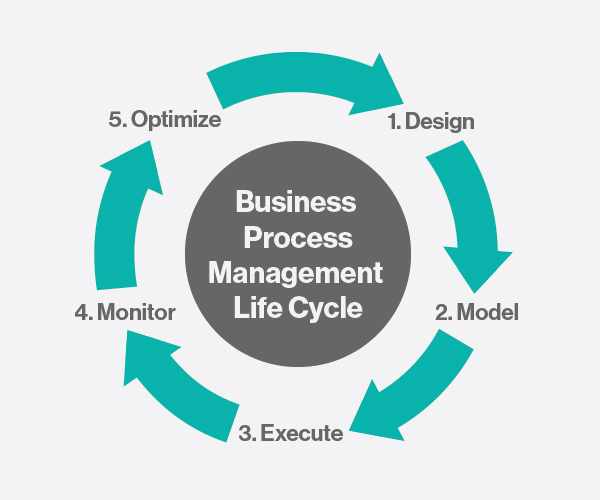
\includegraphics[width=0.6\textwidth, keepaspectratio]{img/bpm-lifecycle.jpg}
    \caption{BPM Life-cycle \cite{harvey-koeppel-bpm-lifecycle-2015}}
    \label{fig:bpm-lifecycle}
\end{figure}

\begin{description}
	\item[Design] -- The requirements of the business are collected, analysed and specified. The specification can be ``as is'' (state of how processes currently are) or ``to be'' (how processes would be). Accompanying graphical materials (such as flow-charts) are included.
    \item[Model] -- Specification is expressed (modelled) with graphical notation \gls{bpmn}, which will be investigated later.
    \item[Execute] -- Changes are implemented and deployed.
    \item[Monitor] -- After deployed changes, monitoring system comes to the scene. Processes are monitored and \gls{bpms} tools are used to collect data and analyse performance through metrics - called \gls{kpi}. \gls{kpi} are defined, optimized metrics which can help to understand the performance of the current business. As an example of \gls{kpi} can be ``an average number of requests for new order per day'' and many more, individual metrics to concrete business.
    \item[Optimize] -- At some point, when an appropriate number of data are collected and analysed with monitoring, optimization is done. The goal of optimization is to find issues or some improvements. After that, new specifications and improvements are created and \textit{design} stage is executed again.
\end{description}
% -------------------------------------------------------------------------------
\subsection{Business Process Model and Notation}
\gls{bpmn} is notation created and standardised by \textit{Object Management Group} (see \url{https://www.omg.org}). According to~\cite{bpmn-org-2018} \gls{bpmn} can be described as:
\begin{quote}
  \gls{bpmn} is a graphical notation that depicts the steps in a business process. BPMN depicts the end to end flow of a business process. The notation has been specifically designed to coordinate the sequence of processes and the messages that flow between different process participants in a related set of activities.
\end{quote}
The notation itself, elements which are used and how modelling is done, are not described. For this information, see~\cite{bpmn-org-2018}.
% -------------------------------------------------------------------------------
\section{Business Intelligence}

\gls{bi} is a way how business can collect an enormous amount of data, structure them and analyse (see \cref{fig:bi-diagram}. From \gls{bpm} life-cycle view, \gls{bi} is a \textit{Monitor} stage. Systems which are tagged as \gls{bi} tools typically offers some kind of reporting, dashboards and scorecards. 

\begin{figure}[ht!]
	\centering
    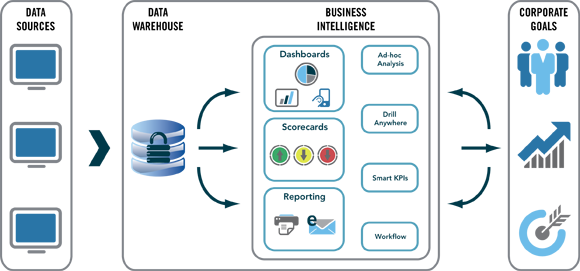
\includegraphics[width=0.6\textwidth]{img/mortgage-business-intelligence-diagram.png}
    \caption{Business intelligence diagram \cite{business-intelligence-diagram-2018}}
    \label{fig:bi-diagram}
\end{figure}

\textbf{Dashboard} offers graphical overviews of collected data. Dashboards are typically highly customizable and can offer different types of views for each employee to help achieve their job. Dashboards can help understand and find issues within business and potentially more quickly solve them. \Cref{fig:bi-dashboard} shows an example. 

\textbf{Scorecards} offer monitoring of \gls{kpi} metrics and user can easy compare goals and current results. Scorecards also easily show performance of business, for example if business plan is fulfilled or financial flow (e.g if business is profiting or not,\dots). 

\begin{figure}[ht!]
	\centering
    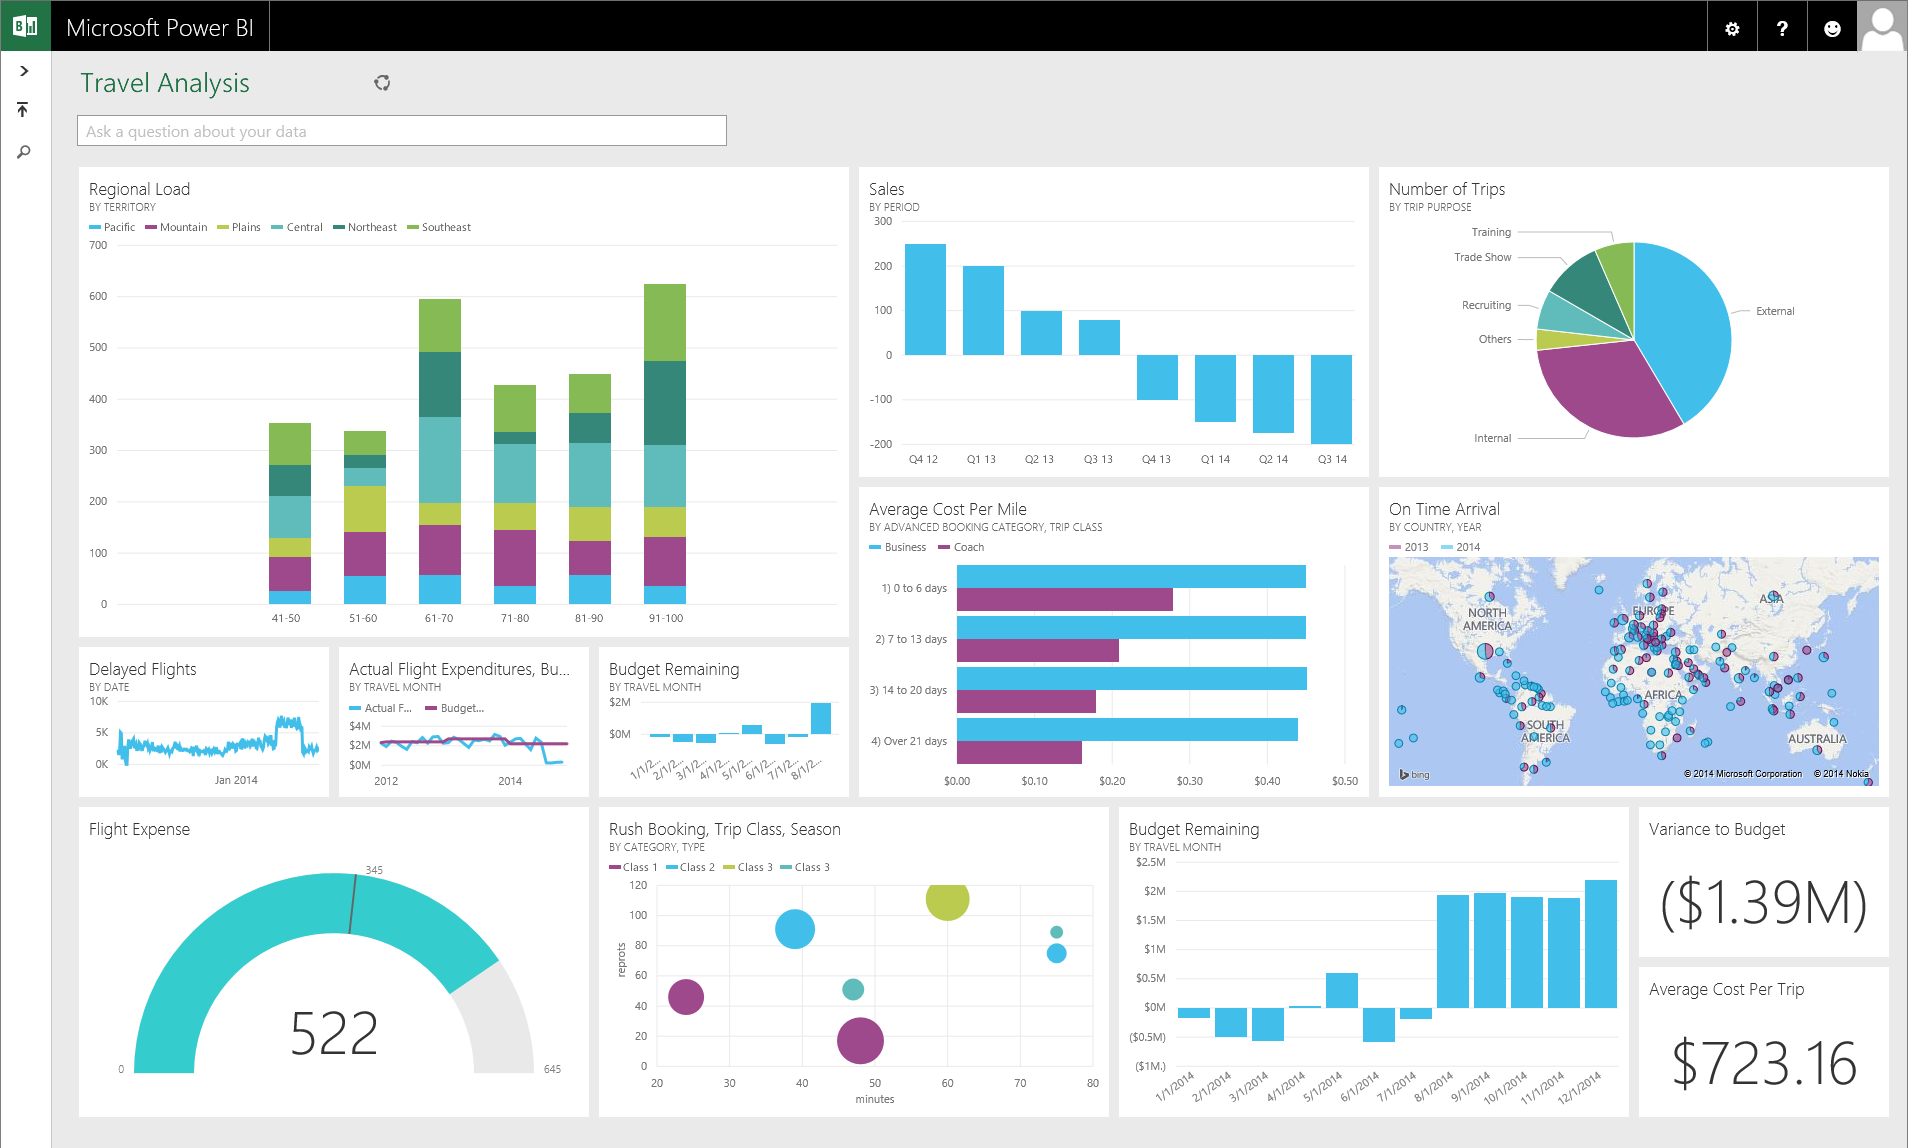
\includegraphics[width=0.6\textwidth]{img/microsoft-power-bi-dashboard.png}
    \caption{Business Intelligence dashboard example~\cite{ms-business-intelligence-2018}}
    \label{fig:bi-dashboard}
\end{figure}
% -------------------------------------------------------------------------------
\section{Enterprise ontology}
According to~\cite{gruber-translation-1993}, definition of ontology states as ``An ontology is a specification of a conceptualization''. In other words ontology is description, a formal specification, of concepts and relationships.

Enterprise Ontology~\cite{dietz-essence-2015} is the understanding of the essence of organisation, completely independent of the way in which this essence is realised and implemented.

The DEMO Methodology~\cite{dietz-enterprise-2006} is an engineering methodology, based on theory of enterprise ontology.

The following text was taken from article describing \gls{eo} theory~\cite{haan-modeling-2009}:

\begin{quotation}
Enterprise ontology is focused on the essence of the operation of an organization, meaning that it is fully independent of the (current) realization and implementation of the organization. The theory that underlies the notion of enterprise ontology as presented by Dietz is called the PSI-theory. Dietz uses this theory to construct a methodology providing an ontological model of an organization, i.e. a model that is coherent, comprehensive, consistent, and concise, and that only shows the essence of the operation of an organization model. This methodology is called \gls{demo}.

Compared to its implementation model, the ontological model of an enterprise offers a reduction of complexity of over 90\%. This reduction of complexity makes an organization for a manager intellectual manageable and transparent. It also shows the coherence between all fields within the enterprise, like business processes, workflow, organization structure, etc.

The overall goal of the PSI-theory (the theory behind the notion of Enterprise Ontology) is to extract the essence of an organization from its actual appearance. It presents four axioms that help to achieve this goal.

The \textbf{operation axiom} (\cref{fig:OperationAxiom}) tells us that the implementation independent essence of an organization is that it consists of subjects fulfilling actor roles. A subject fulfilling a certain actor role is called an actor. Actors constitute the operation of an organization by performing two kinds of acts: production acts and coordination acts.

\begin{figure}[ht!]
	\centering
    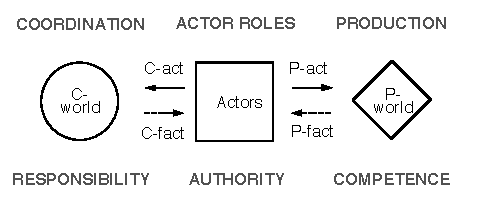
\includegraphics[width=10cm, keepaspectratio]{img/OperationAxiom}
    \caption{The operation axiom \cite{haan-modeling-2009}}
    \label{fig:OperationAxiom}
\end{figure}

By performing production acts (P-acts for short) the subjects contribute to bringing about the goods and/or services that are delivered to the environment of the organization. The results of P-acts are production facts (P-facts for short), which can be divided into material (something is manufactured, stored or transported) and immaterial (decisions or judgements) facts.

By performing coordination acts (C-acts for short) subjects enter into and comply with commitments towards each other regarding the performance of production acts. A C-act is performed by one actor, the performer, and directed to another actor, the addressee. C-acts consist of an intention (e.g. request, promise, question, assertion) and a proposition (the performer proclaims the fact and the associated time the intention is about) and result in coordination facts (C-facts for short).

The \textbf{transaction axiom} tells us that C-acts are performed as steps in universal patterns, called transactions. This axiom reveals universal socionomic patterns of coordination that hold for all organizations. The standard transaction pattern is shown in~ \cref{fig:TransactionPattern}. A white box represents a C-act type and a white disk represents a C-fact type. A gray box represents a P-act type and a gray diamond a P-fact type. 

\begin{figure}[ht!] 
	\centering
    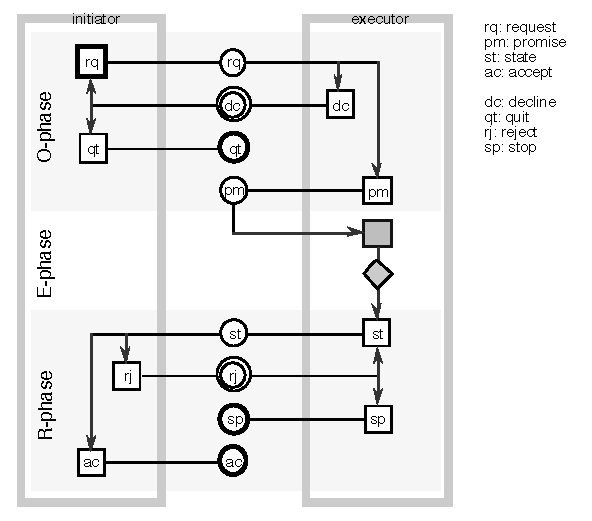
\includegraphics[width=8cm, keepaspectratio]{img/TransactionPattern}    
    \caption{The standard transaction pattern \cite{haan-modeling-2009}}
    \label{fig:TransactionPattern}
\end{figure}

Two actors are involved in a transaction, the initiator and the executor. A transaction evolves in three phases: the order phase (O-phase for short), the execution phase (E-phase for short), and the result phase (R-phase for short).

The \textbf{composition axiom} tells us how P-facts are interrelated. It states that every transaction is enclosed in some other transaction, or is a customer transaction of the organization under consideration, or is a self-activation transaction. According to Dietz this axiom provides the basis for a well-founded definition of the notion of business process.

The \textbf{distinction axiom} (\cref{fig:DisctinctionAxiom}) tells us that actors exert three basic human abilities: performa, informa, and forma. Through the distinction axiom a substantial reduction of complexity and diversity is achieved, regarding both the coordination and the production in an organization.

\begin{figure}[ht!]
	\centering
    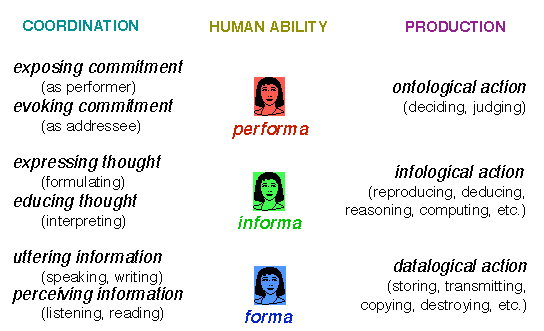
\includegraphics[width=10cm, keepaspectratio]{img/DistinctionAxiom}
    \caption{The distinction axiom \cite{haan-modeling-2009}}
    \label{fig:DisctinctionAxiom}
\end{figure}
% -------------------------------------------------------------------------------
\subsection{The Organization Theorem}

The organization theorem combines the benefits of these axioms into one concise, comprehensive, coherent, and consistent notion of enterprise. This theorem states that the organization of an enterprise is a heterogeneous system that is constituted as the layered integration of three homogeneous systems: the B-organization (from Business), the I-organization (from Intellect), and the D-organization (from Document). Figure~ \ref{fig:OrganizationPyramid} visualizes the organization theorem and shows us that the D-organization supports the I-organization, which supports the B-organization. The coordination parts of these three systems are similar, they only differ in the kind of production: the production of the B-organization is ontological, the production in the I-organization is infological, and the production in the D-organization is datalogical.

\begin{figure}[ht!]
	\centering
    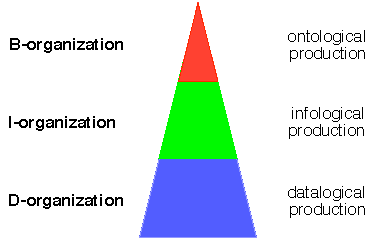
\includegraphics[width=6cm, keepaspectratio]{img/OrganizationPyramid}
    \caption{The organization theorem \cite{haan-modeling-2009}}
    \label{fig:OrganizationPyramid}
\end{figure}

\end{quotation}
% -------------------------------------------------------------------------------
\section{Modelling with DEMO}
In this section, firstly short description of modelling aspects is provided and then a illustrative example how modelling with \gls{demo} can be more precise and shorter than creating model with \gls{bpmn}. 

All used elements in DEMO modelling are described in aspects models arranged as pyramid. However the two core elements are Ontological transaction and Actor roles. Good summarization of these two core elements are from master thesis by Zuzana Vejrazkova~\cite{vejrazkova-demo-2013}:

\begin{quote}
	\begin{description}
		\item[Ontological transaction] -- Involves actions that happen on the ontological level, as described by the Distinction axiom. Those involve bringing about the facts that did not exist before, making decisions, or transporting physical elements. Completion of a transaction, in a way that is described by the transaction axiom, results in a new original fact, called the P-fact.
        \item[Actor role] -- There are two actor roles, the initiator and the executor. They play an important role in DEMO modelling, as each transaction needs to have exactly one initiator and one executor. On the implementation level, 1~person can (and often does) posses more actor roles.
	\end{description}
\end{quote}

Figure \ref{fig:DemoAspectModels} shows that ontological model can be divided to four sub-models. The good and brief explanation is in the book \textit{The essence of organisation: an introduction to enterprise engineering}~\cite{dietz-essence-2015}:

\begin{figure}[ht!]
	\centering
    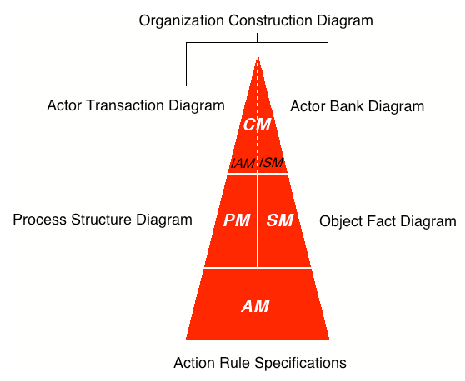
\includegraphics[width=8cm, keepaspectratio]{img/DemoAspectModels}
    \caption{The DEMO Aspect Models pyramid \cite{dietz-discipline-2013}}
    \label{fig:DemoAspectModels}
\end{figure}

\begin{quote}
	\begin{description}
		\item[Construction model] (CM) is the most concise sub-model. Therefore it is put at the top of the triangle. An additional meaning of this position is that there is nothing ``above'' the CM. The Construction Model shows the identified transaction kinds, the corresponding actor roles, and the border of the Scope of Interest.
         \item[Action model] (AM) is the most comprehensive one, in the sense that the other three may be derived from it. The AM of an organisation consists of the action rule specifications for every internal actor role. Action rules are guidelines for dealing with the events that actors have to respond to.         
         \item[Process Model] (PM) shows precisely how the identified transactions are interrelated in tree structures. These tree structures are what people commonly refer to as business process models.         
         \item[Fact Model] (FM) show the fact kinds in the production world of the organisation and their interrelationships. 
	\end{description}
\end{quote}

\begin{figure}[ht!]
	\centering
    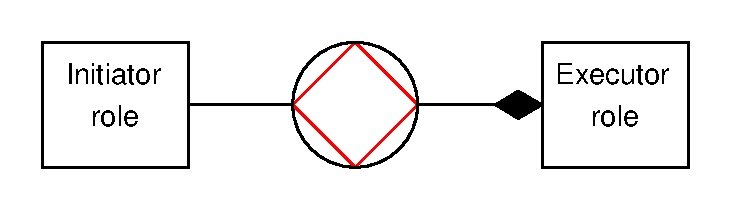
\includegraphics[width=6cm, keepaspectratio]{img/ocd-symbol-example}
    \caption{The core OCD element - transaction symbol with assigned actor roles}
    \label{fig:ocd-symbol-example}
\end{figure}

The PM is in between CM and the AM, that means it is more detailed than CM but less than AM. The PM and the FM are on the same layer of the pyramid and it refers to the fact, that PM takes the process view of coordination world, and the FM is for the production world in the same meaning as PM.

From the CM is used \gls{ocd} which takes standard process pattern and squeeze it to one symbol with two connected boxes which represent initiator and executor actor roles (see \cref{fig:ocd-symbol-example}).

From the PM is taken \gls{psd} sub-model which describes business processes and the exact way how each transaction is connected with another. Following explanation how \gls{psd} is modelled is from~\cite{dietz-essence-2015}:

\begin{quote}
      The disk of the transaction is stretched horizontally, such that it looks like a sausage. One must imagine that there is an invisible and non-proportional time line from left to right (promise is performed after its request,\dots). Coordination acts and facts are represented by small boxes and disks on the border of the transaction symbol (the sausage). 
      The production act, execute, is represented by a small grey box on the edge of the production symbol. To the left of it is the order phase, and to the right the result phase.
      Between two transactions (the sausages) can be added arrows, either solid or dashed. Solid arrows represent \textit{response links}. Response link means that the act at the arrow point is performed in response to the event at the shaft. Dashed arrow represent \textit{waiting links}. Their meaning is that performing the act at the arrow point must wait for the event at the shaft having occurred. Through ``swim lanes'' the responsibility areas of the actor roles are indicated.
\end{quote}
An example of PSD is shown at \cref{fig:psd-example} which means exactly ``When the transaction T1 (Supply order) is \textit{requested}, as a response, T2 (Tax payment) is also \textit{requested}. After that, T1 can be promised only and only, if T2 is \textit{accepted}. After that T1 can be completed''.

\begin{figure}[ht!]
	\centering
    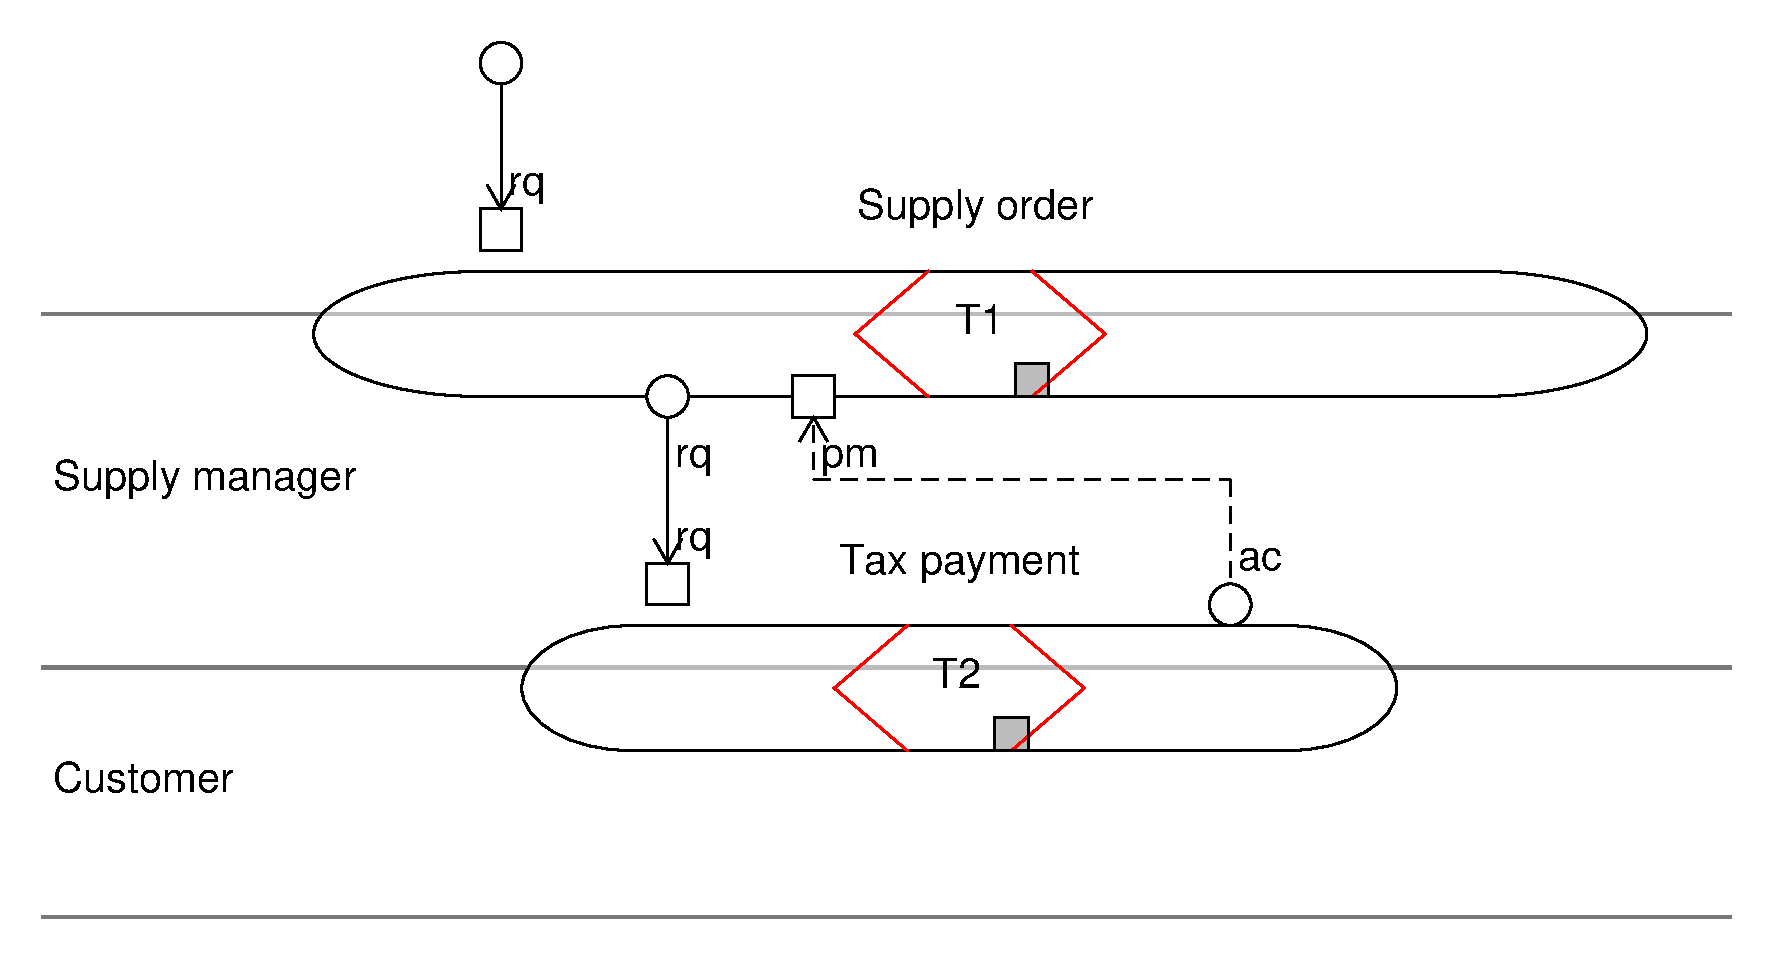
\includegraphics[width=0.7\textwidth]{img/psd-example}
    \caption{PSD example}
    \label{fig:psd-example}
\end{figure}
% -------------------------------------------------------------------------------
\subsection{Advantage of DEMO Over BPMN}    
\gls{bpm} notation is well defined, established and widely used. Many \gls{bpm} solutions exist around and of course, \gls{bpmn} is used ``under the hood''. These systems will be described later in \cref{ch:bpms}.

One thing is absolutely clear, with enlarging business requirements, the business processes "grow up" too and so \gls{bpmn} diagrams. This can lead to very large and complex diagrams, which can be harder to read and understand. One of the advantages of DEMO is the fact, that same \gls{bpmn} diagram can be represented within DEMO notation. The result is reduced complexity with the same understanding as diagram within \gls{bpmn}. However, advantages of DEMO notation can be used not only within \gls{bpmn}. For example, students at subject MI-MEP (Modelling economic processes, translated) at \gls{ctu}~\cite{ccmi-2018} transferred large Trump's flow chart\cite{quartz-trump-2017} (about highway building process) to DEMO OCD diagram. The flow chart that fills several pages, \gls{demo}'s \gls{ocd} fills only one page of size A4. 
To summarize, DEMO can really help to better understand business processes without too much complexity of diagrams itself.
% -------------------------------------------------------------------------------
\section{Gantt chart}
According to~\cite{gantt-chart-2018}, Gantt chart was proposed in 1890 by Karol Adamiecki, but he did publish his work only in the Polish language. About the year 1910 American engineer, Henry Gantt, introduced his own version of this chart and this work became widely used and is still used by project managers. 
Gantt chart serves as an overview of activities according to the time schedule. By simplicity, Gantt chart shows, what has to be done (an activity) and when.
At \cref{fig:gantt-chart-example} is an example of Gantt chart. The core element is some kind of bar chart (progress bar) which starts at some time and is scheduled to end in another time.
Nowadays, Gantt charts, has more advanced elements, such as connected activities (one activity must end before another can start), groups of activities, different colours of activities that can indicate different phases of completion and so on. Many systems for time-management support these types of graphs.
Gantt chart and its usage for this thesis are discussed later, in chapter \cref{ch:proposed-approach}.

\begin{figure}[ht!]
	\centering
    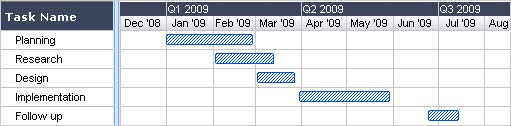
\includegraphics[width=0.8\textwidth]{img/gantt-chart-example.jpg}
    \caption{Gantt chart example \cite{gantt-chart-2018}}
    \label{fig:gantt-chart-example}
\end{figure}



\chapter{Process Visualisation}
\label{ch:bpms}
\todo{intro}
\section{State of BPMS Solutions}


\begin{figure}[ht!]
	\centering
    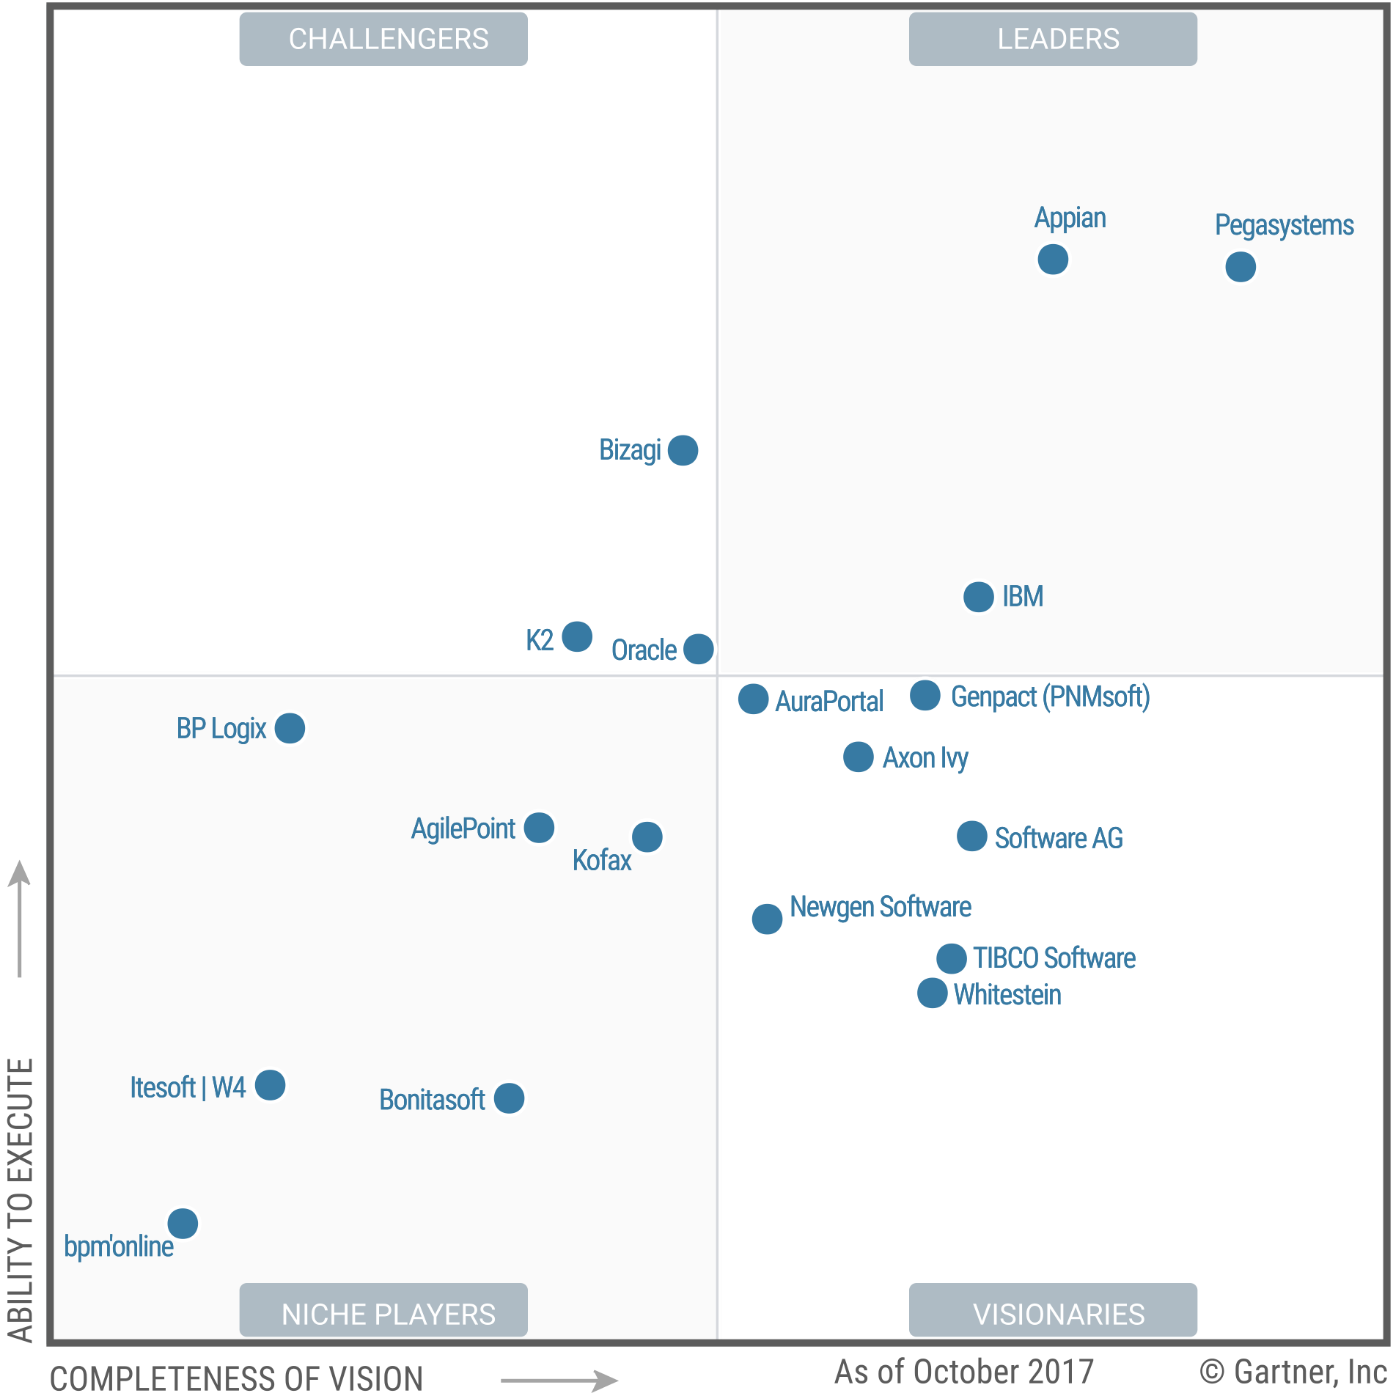
\includegraphics[width=0.6\textwidth, keepaspectratio]{img/gartner-magic-quadrant.png}
    \caption{Gartner Magic Quadrant\cite{gartner-2017} }
    \label{fig:gartner-magic-quadrant}
\end{figure}

Nowadays \gls{bpms} software supports all stages of \gls{bpm} life-cycle (design, modelling, execution, monitoring and optimization). These systems also offer real-time collaboration, integration with cloud and mobile devices. Many systems also integrate artificial intelligence - for predictive analysis or some automatic decisions. \gls{bpms} software allows to create highly productive application, where is no need to manual implementation of business rules. \gls{bpms} includes defining processes, data models and also user interfaces. Also highly customized monitoring stage is included, which means users can customize \gls{kpi} metrics, appearance of dashboard and so on. On top of that functions, some solutions have ability to display (visualise) current running processes.  

Result is typically web based application which employees can use to do their jobs without knowing that there are some defined processes and layer of some BPM software. 

According to \textit{Gartner Magic Quadrant}\cite{gartner-2017}, the most used systems are \textit{Appian}, \textit{Pegasystems}, \textit{IBM} and many more as shown at~\cref{fig:gartner-magic-quadrant}.

 \subsection{Closer Look at Process Maker}
 
 \textit{ProcessMaker} (\href{https://www.processmaker.com/}{https://www.processmaker.com/}) is web-based \gls{bpm} solution which allows to build, run, monitor and optimize business processes. Building of processes is done via \gls{bpmn}. Inside designer %(see \cref{fig:process-maker-designer},
 users can define data sources (variables) which will be used later within running processes. 
 
%  \begin{figure}[ht!]
% 	\centering
%     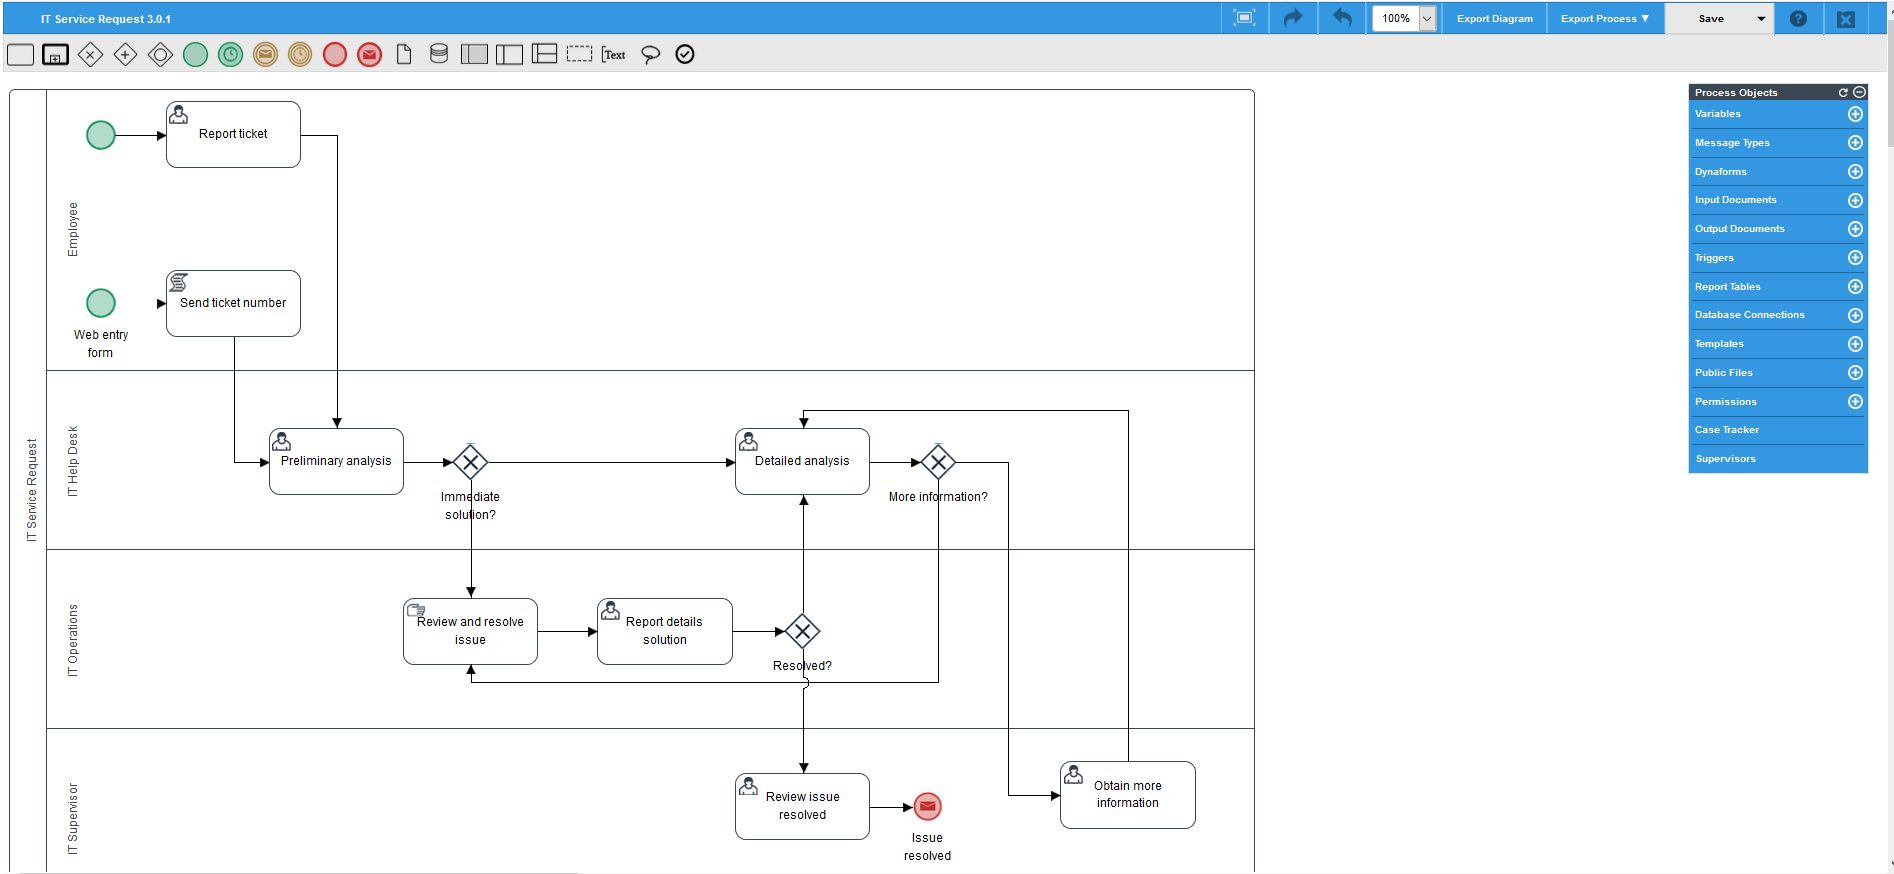
\includegraphics[width=0.8\textwidth, keepaspectratio]{img/process-maker-designer.PNG}
%     \caption{ProcessMaker designer}
%     \label{fig:process-maker-designer}
% \end{figure} 
 
\begin{figure}[ht!]
    \centering
    \subfloat{{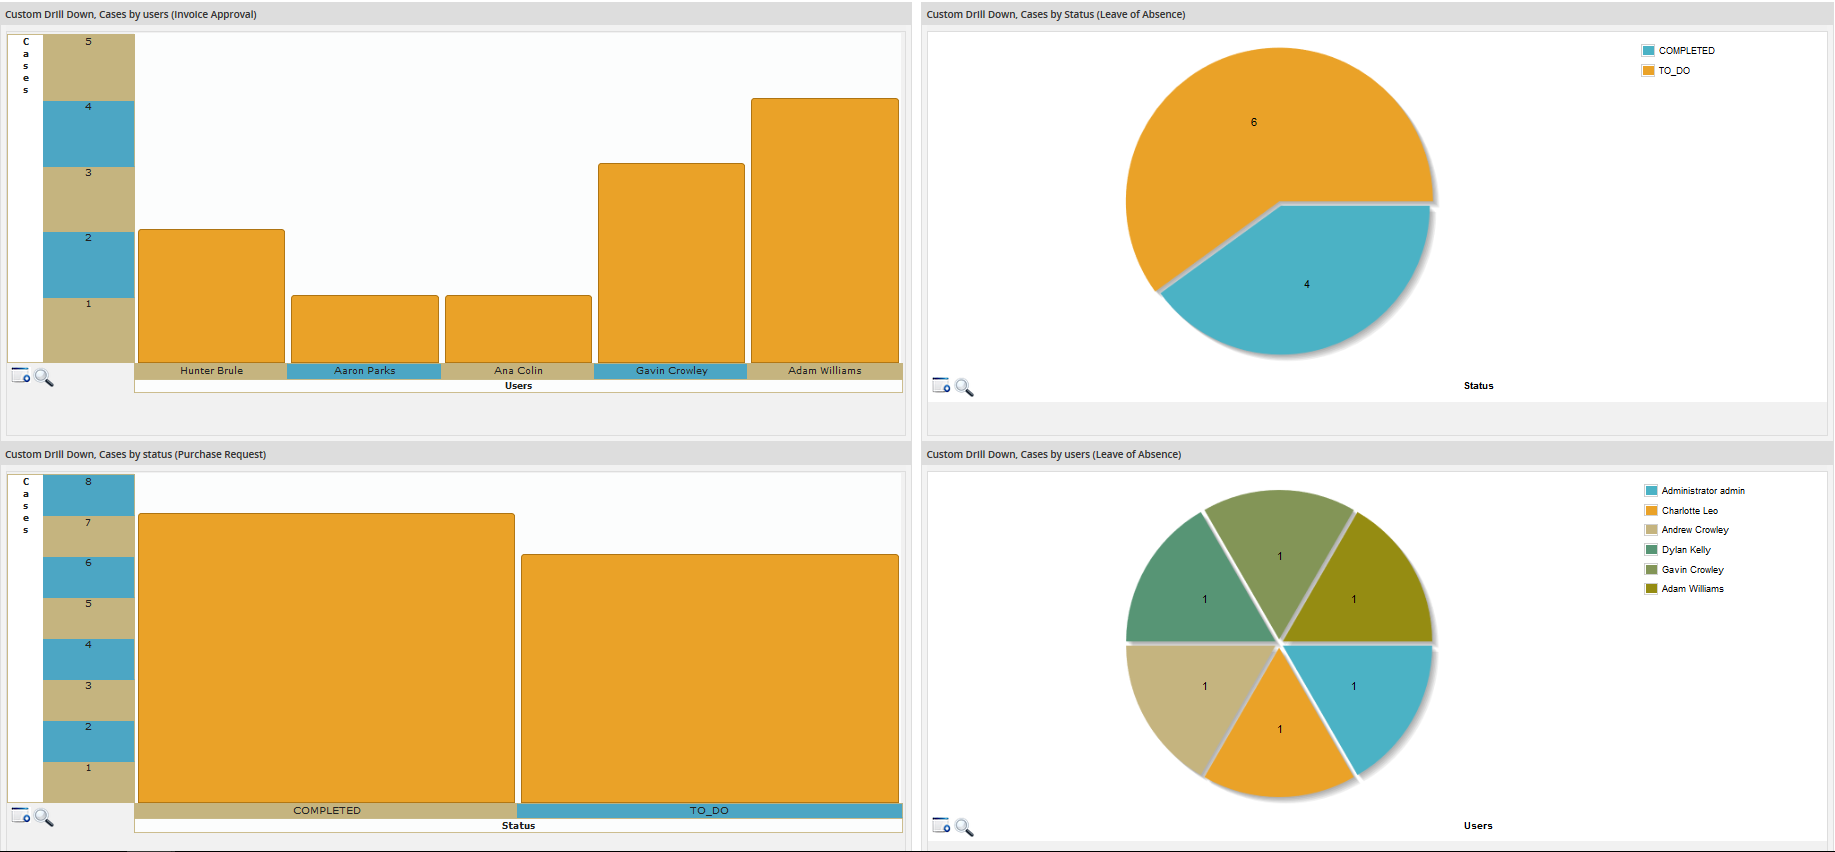
\includegraphics[width=10cm, keepaspectratio]{img/process-maker-dashboard.PNG} }}%
    \qquad
    \subfloat{{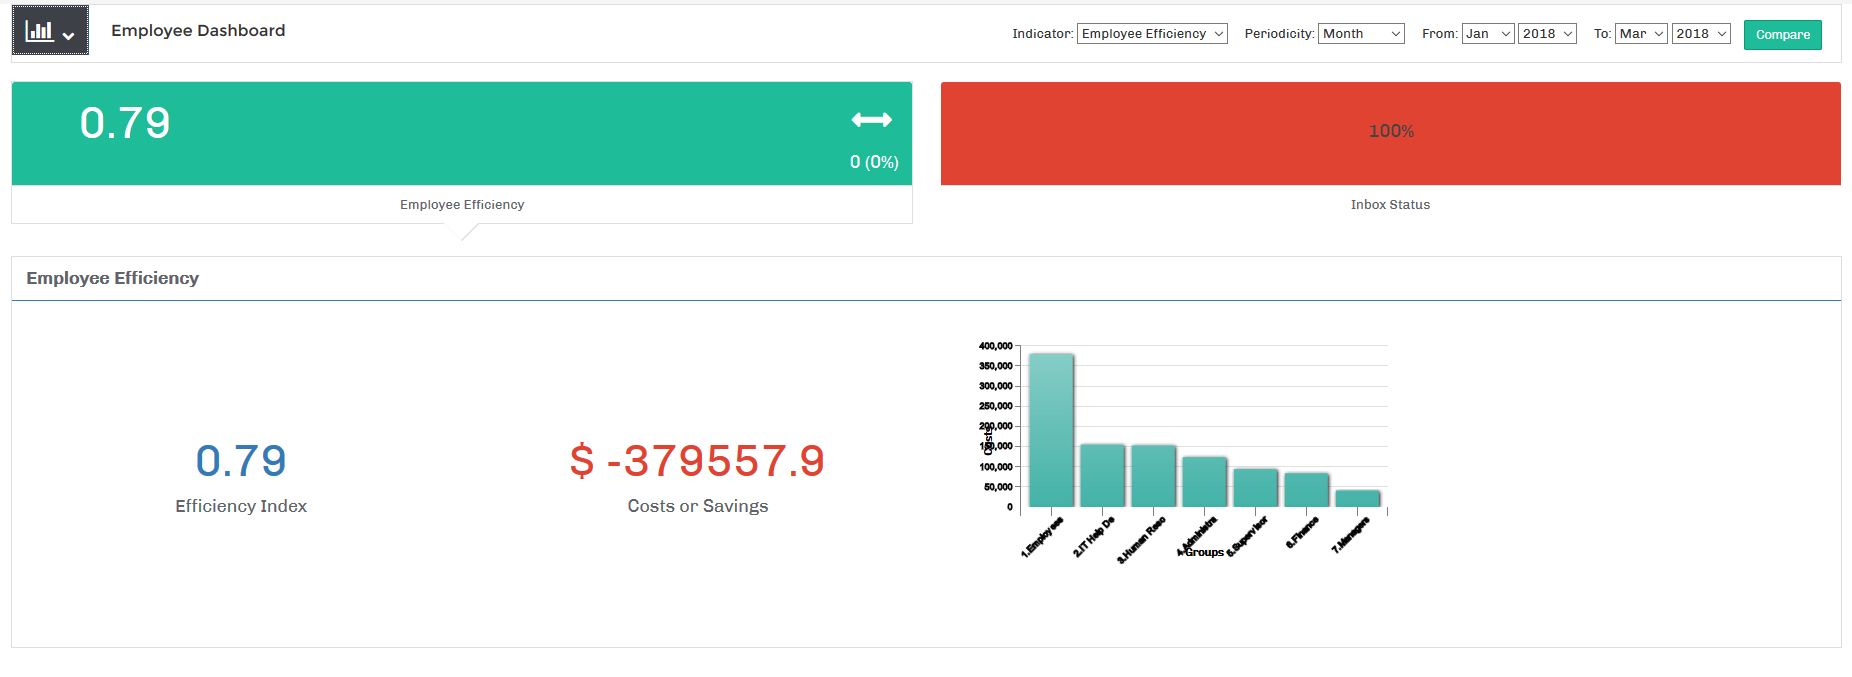
\includegraphics[width=10cm, keepaspectratio]{img/process-maker-employee-kpi.PNG} }}%
    \caption{ProcessMaker dashboard and KPI examples\todo{cite}}%
    \label{fig:process-maker-dashboard}%
\end{figure}

 After process is designed and variables defined, next step is to define user interface, called DynaForms. End users interact mainly with \textit{DynaForms}, where they fill appropriate pieces of data. 
 Inside designer of \textit{DynaForms}, user connects data fields with variables from defined processes. Also user can define input or output documents for processes or define events (called triggers) what will happen when some kind of event occurred.
 
 When processes are defined and \textit{DynaForms} created, processes can be deployed. After deploy, \gls{kpi}s and dashboards can be managed. \textit{ProcessMaker} offers creating custom metrics, which will be precise to business requirements and customize dashboards. Many of graphs are interactive, which can display more detailed information. An example is shown at \cref{fig:process-maker-dashboard}.
 
 \begin{figure}[ht!]
	\centering
    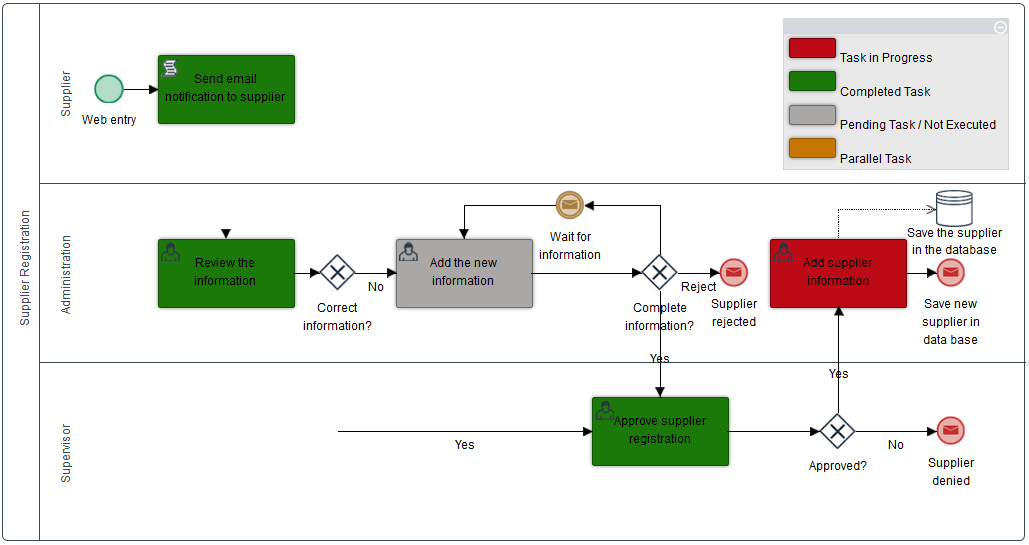
\includegraphics[width=10cm, keepaspectratio]{img/process-maker-map.PNG}
    \caption{ProcessMaker process map\todo{cite}}
    \label{fig:process-maker-process-map}
\end{figure} 
 
 From end-user view, \textit{ProcessMaker} (as many others \gls{bpms}) behaves as web-based application, which allows to do his job via predefined \textit{DynaForms}. ProcessMaker moreover offers process map, which is graphical visualisation of running process. Process map is in \gls{bpmn} and each activity element has different colour to indicate its state (\cref{fig:process-maker-process-map}).
 
\subsection{Process Simulation and Analysis}
Another tool, \textit{Bizagi Modeler} (\href{https://www.bizagi.com/uk/products/bpm-suite/modeler}{https://www.bizagi.com/uk/products/bpm-suite/modeler}), offers modelling processes with \gls{bpmn} and run simulations on top of them.

\textit{Bizagi Modeler} for simulations defines scenarios. Each scenario has many attributes, but mainly:
\begin{description}
    \item[Resources] Resource is some entity (e.g. customer, employee role, equipment) which is used to define how each task of the process uses these resources (e.g. task verification uses resource ``Inspection agent'').
    \item[Time consumption] For each task users can define how much time is consumed to complete. Consumption can be defined as simple (constant) number or with the probability distribution.
    \item[Cost] Users can define for tasks how much execution cost (in a financial way).    
\end{description}

For gateways (element from \gls{bpmn}) users can define probability next flow (e.g. probability for ``yes'' than ``no''). \textit{Bizagi Modeler} has different levels of simulations.
    \begin{description}
        \item[Process validation] User defines a duration of simulation and amount of generated instances (number of requests). Gateways are also configurable. After simulation ends, the result with summarization is displayed and the user can check if process behaves as expected. For example, if the number of requests is equal to the number of completed instances. This could occur if there are issues with synchronization with parallel gateways.
        \item[Throughput time analysis] Focuses only on time measurement and resources are not included. The user defines consumption for requests (interval time between two instances can be generated) and also for every task (how much time task gets to complete). Analysis counts total completed tasks and also average time and total time spent on each task. For example, it is useful for predictions, e.g. ``how long customer will wait until his request is completed''.
        \item[Resource analysis] Users can define resources and how much resource costs (fixed or cost per hour). Each task has defined which resources need and how much to execute. Also, the cost of each task and time consumption are included. This analysis is more complex and serves as the real-world simulation to achieve better results, which can help to optimize processes. A simulation results example is shown at \cref{fig:bizagi-example}.
    \end{description}

\begin{figure}[ht!]
    \centering
    \subfloat{{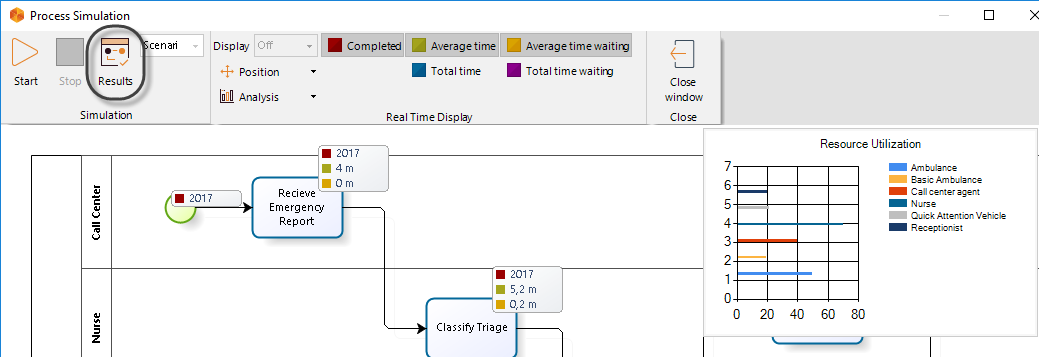
\includegraphics[width=10cm, keepaspectratio]{img/bizagi-process-simulation.png} }}%
    \qquad
    \subfloat{{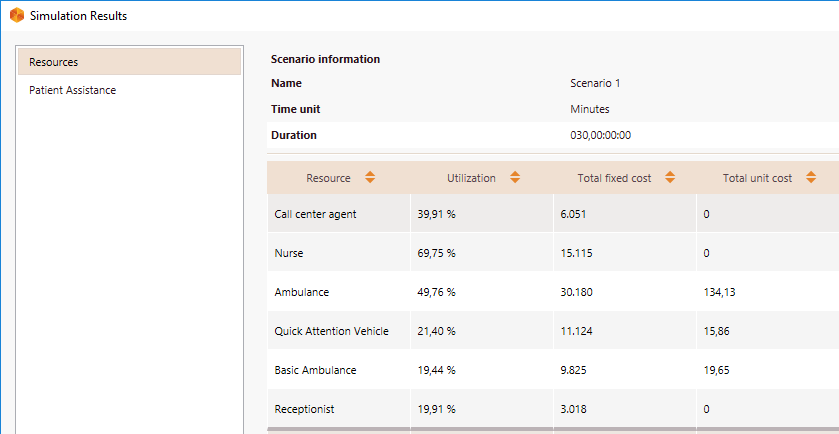
\includegraphics[width=10cm, keepaspectratio]{img/bizagi-simulation-results.png} }}%
    \caption{\textit{Bizagi Modeler} Resource analysis example\cite{bizagi-2018}}%
    \label{fig:bizagi-example}%
\end{figure}

% In this section a more details how \gls{bpms} works were provided. A two concrete solutions were shown and briefly described. These two systems became base inspiration for providing similar functionalities to \gls{bpms} based on DEMO (from now called \textit{Demo Machine}) . In the next section follows summarization, how DEMO Machine could work and how data could be aggregated and prepared to 
% visualisation.  

\section{BPMS Architecture}
The common \gls{bpms} architecture is shown at~\cref{fig:bpms-architecture}. Business analysts and process developers design process models and deploy them within \gls{bpms} solution. Users (process participants) has access to unified user interface which is connected with all layers of \gls{bpms}. On the right side of overview, the \textit{monitoring} stage of \gls{bpm} stage is included. Users has access to highly precious collected data through graphical views. They can more easily determine what happens and decide what next steps could be to make their business even better. 

\begin{figure}[ht!]
	\centering
    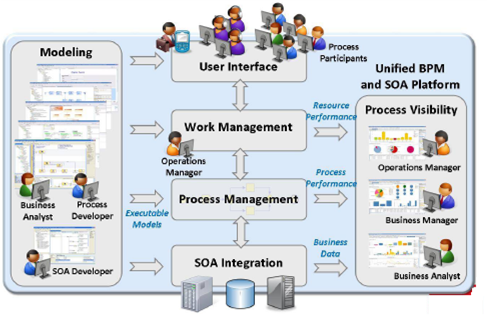
\includegraphics[width=12cm]{img/tibco-bpm-architecture.png}
    \caption{BPMS Architecture\cite{tibco-bpm-2016}}
    \label{fig:bpms-architecture}
\end{figure}

\section{DEMO Role within Business Intelligence}
The thesis focuses on ``Business Intelligence'', in other words on the fourth stage of \gls{bpm} life cycle. The goal is to provide an approach which can more precisely describe business processes and connections between collected data and these processes. In \cref{ch:theoretical-foundations} the \gls{demo} methodology was introduced and explained. Describing business processes from collected data within enterprise solution with \gls{demo} brings mainly these advantages: 
\begin{enumerate}
\item Consistency -- within \gls{demo} the models are consistent. 
\item Clear assignment of responsibility -- within \gls{demo}, each transaction has clearly defined the responsibility of actor roles. 
\item Reduced complexity –- there is only and only one way how to describe an enterprise within DEMO.
\end{enumerate}

The first stage of \gls{bpm} life-cycle (design) within \gls{demo} is well described by Dietz\cite{dietz-essence-2015}\cite{dietz-enterprise-2006}. However next stages of \gls{bpm} life-cycle are only theories ``on paper'' and they are not stated to practice. For example, \textit{M. Skotnica}\cite{diploma-skotnica-2016} with his thesis focused on first three stages and introduced an approach of \gls{bpms} based on \gls{demo}. But the next stages are not examined yet.

This thesis focuses on fourth stage (the monitoring) and the premise is that underlying \gls{bpms} solutions are not necessary based on \gls{demo}. The goal is to aggregate data from any enterprise solution, connect them with modelled enterprise within \gls{demo} methodology and display them to the user. The main difference is with the feature of process visualisation itself. Systems based on \gls{bpmn} visualise processes within \gls{bpmn} which, as was told, can be more complex, inconsistent and not so clear as approach with \gls{demo}. 

In this chapter, firstly more details about \gls{bpms} were provided. On the two concrete solutions available were taken the core concepts of process modelling and their visualisations. The role of \gls{demo} within \gls{bpms} and Business Intelligence was explained. In the next chapter, the proposed approach itself is introduced and described.




\chapter{Proposed Approach}
\label{ch:proposed-approach}
The main goal of the thesis is to propose an approach which will be able to create the graphical overviews of critical business data and make decisions based on them. This chapter describes each part of the proposed approach. The chapter is divided to these parts:	
    \begin{enumerate}
      \item Which kind of data the application collects and how works with them.
      \item How real-time process visualization is done.
      \item What kind of overviews the application can display. 
    \end{enumerate}
% -----------------------------------------------------------------------
\section{Business Data Aggregation}
Each enterprise system collects precious data within business. These data are important in many ways. One is for business analysts. Analyst can with these collected data analyse processes and optimize them. Although every enterprise solution has differently defined structure of these data and every \gls{bpms} has different approach how it works with them, the core concept of how data can be described remains the same. 
Within \gls{bpms} there are elements which can be transformed always to the \gls{demo} concepts.
\begin{itemize}
\item There are always some kind of \textit{Actor roles} and concrete \textit{Actors}. Commonly \gls{bpms} defines \textit{Actor roles} as ``roles'' and \textit{Actors} defines as ``users''.
\item The processes itself can be transformed to \textit{Transactions}. In~\cref{ch:theoretical-foundations} was explained that each process can be described on ontological level and has precise definition what kind of process it is and the responsibilities of \textit{Actors}.
\item Each \gls{bpms} provides some kind of events, which can be used to determine what exactly happened and how it is connected to the model defined within \gls{demo}.
\end{itemize}

\begin{figure}[ht!]
  \centering
  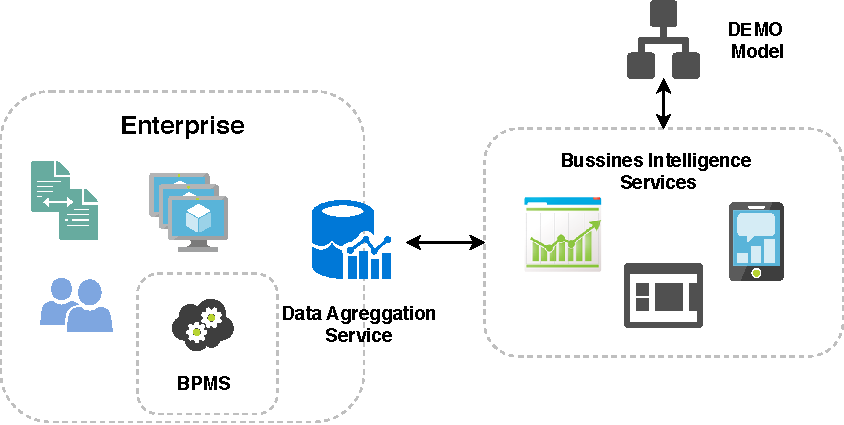
\includegraphics[width=12cm,keepaspectratio]{img/bi-demo-overview}
  \caption{Business Intelligence based on DEMO}
  \label{fig:bi-demo-overview}
\end{figure}    

In this way the system of visualisation based on \gls{demo} can be nearly independent from other systems within enterprise. The architecture of Business Intelligence based on \gls{demo} is shown at~\cref{fig:bi-demo-overview}. The enterprise does not need necessary a \gls{bpms}. Within enterprise, many systems and applications exists. Even without BPMS solutions within enterprise there are still the same kind of processes and actor roles which can be modelled through \gls{demo}.

Inside an enterprise there can be many systems and (not necessary) in front of them can be a \gls{bpm} solution. On the ``borders'' of the \textit{Enterprise} is placed \textit{Data Aggregation Service}. This service has responsibility of getting data from an \textit{Enterprise} and transforming them to the structure that \textit{Business Intelligence Services} can use. Collected data from \textit{Data Aggregation Service} are mapped to defined \textit{DEMO Model}.
With this approach, \textit{Business Intelligence Services} can take advantages of \gls{demo} without requirement to be dependent directly on enterprise systems.
% ----------------------------------------------------------------------------------------
\subsection{Business Data Domain Model}
\begin{figure}[ht!]
  \centering
  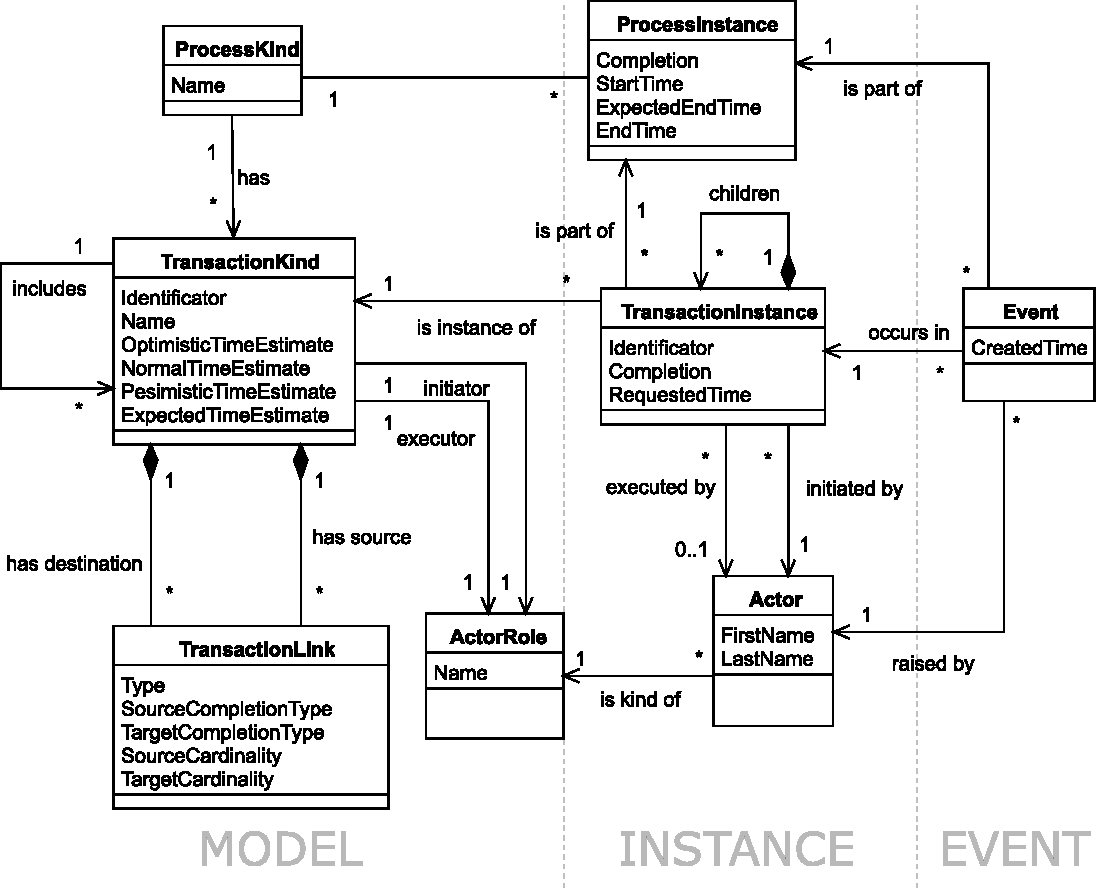
\includegraphics[width=13cm,keepaspectratio]{img/domain-data-model}
  \caption{Domain model of collected data}
  \label{fig:domain-data-model}
\end{figure}    

The one of the most important thing what needs to be defined is how collected data can be expressed for visualisation. The \cref{fig:domain-data-model} shows domain-data model which describes how \gls{demo} model can be described.  

\Cref{fig:domain-data-model} is divided to three parts:
\begin{description}
\item[Model] -- Defines how \gls{demo} model can be described. It corresponds with \gls{ocd} and \gls{psd} models.
\item[Instance] -- The one concrete running process. It indicates state of transactions. 
\item[Event] -- Last part defines the concrete occurred events from internal systems which can be collected and transformed to data, that can be used. 
\end{description}

The brief explanation of each entity from domain model:
\begin{description}
\item[Actor Role] -- Defines role within enterprise. 
\item[Actor] -- Defines concrete user within enterprise, which has assigned \textit{Actor Role}.

\item[Process Kind] -- Defines exactly one concrete business process inside enterprise. Each \textit{Process Kind} has linked amount of \textit{Transaction Kinds}.

\item[Process Instance] -- The instance of concrete \textit{Process Kind}. Defines process \textit{Completion}, date when process instance was created (\textit{StartTime}) and expected time when whole process will be completed (\textit{ExpectedEndTime}).

\item[Transaction Kind] -- Defines the transaction kind. It has linked information, which \textit{Actor Role} is initiator or executor respectively. Also defines the time estimates for transaction completion. These three time estimates -- \textit{Optimistic}, \textit{Normal}, \textit{Pessimistic} are used to compute real expected time. 

\item[Transaction Link] -- Defines the \textit{response} or \textit{waiting} links. Each link has defined \textit{target Transaction Kind}  and \textit{source Transaction Kind} to determine which two \textit{Transaction Kinds} link connects. Link also defines \textit{Source Cardinality} and \textit{Target Cardinality} to define cardinalities. Moreover link defines which \textit{C-Act} is assigned to source and target transactions.  

\item[Transaction Instance] -- Each \textit{Transaction Kind} could have more than one instance. Transaction Instance includes information about \textit{Completion} and \textit{Requested Time}. The instance itself could have more than one children. 

\item[Event] -- An entity to define events which can occur during the running process. Each event has time creation (\textit{Created}) and duration how long it take to between last event and before event was created.

% \item[Completion Changed Event] Event which describes that some C-Act happened within transaction. 
% \item[Initiator / Executor Event] Events which describe that initiator or executor were assigned to \textit{Transaction Instance}. In other words, \textit{Transaction Instance} was initiated or executed by given initiator or executor respectively.
\end{description}
% ---------------------------------------------------------------------------------------

\subsection{A Time Estimate Computation}
Each \textit{Transaction Kind} has three time attributes -- \textit{Optimistic}, \textit{Normal}, \textit{Pessimistic} time estimate. Each one indicates how quickly given task could be completed. These attributes are set manually and it is important decision which values are given. From this three attributes the resulting one is computed.  

Computation is done through technique \textit{Three Point Estimation} \cite{beta-distribution}. 
Manager can take simple average of this three attributes, however the weighted average is more precise.
The following formula comes from \textit{Beta distribution} also known as \textit{PERT}:

\begin{displaymath}
\centering
ExpectedTimeEstimate = \frac{O + 4*N + P}{6}
\end{displaymath}
where (O) states for optimistic, (N) for normal and (P) for pessimistic estimates. It indicates that normal estimate ``can happen'' most likely.
% ----------------------------------------------------------------------------------------
\section{Case Study Rent-A-Car}
Although all proposed approaches are defined generally, the case study is used to demonstrate usage and show examples. The case study is taken from book by J.Dietz~\cite{dietz-essence-2015}. A Rent-A-Car is company which offers cars for rent. The simplified description how company works:

\gls{rac} is a company that rents a cars to persons or a representatives of legal bodies (e.g. companies). \gls{rac} operates from over fifty branches in Europe. Many cities have more than one branch and typically branches are located near all airports. 
Customer orders are placed through several channels: walk-in, telephone, fax or email. Walk-in customers are usually people who want to rent a car immediately. In all cases, an electronic rental form is filled out by one of the desk officers. 
After the renter has signed the contract, the rental is concluded by the desk officer. On the starting day, the driver can pick up a card at the distribution department. When driver shows up, \gls{rac} employee checks whether there is a car available. If there is one, he prepare car and sign contract as being picked up. If there is no car, he will upgrade the contract and select a different car. 
After the car of rental has been dropped off, there is chance to pay some fines. There many types of penalties.

The \gls{ocd} and \gls{psd} of \gls{rac} are shown at~\cref{fig:rac-ocd} and \cref{fig:rac-psd} respectively.
\begin{figure}[ht!]
\centering
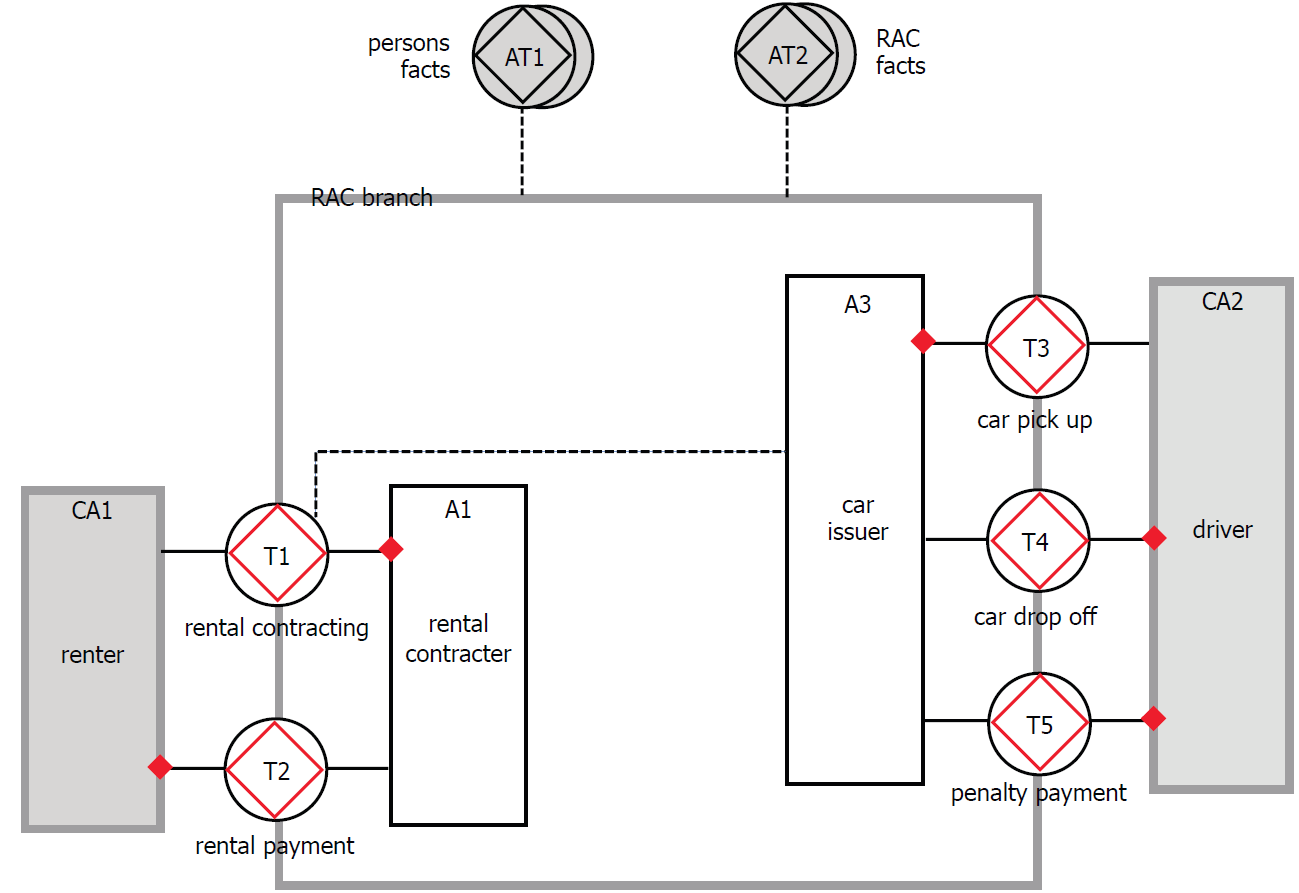
\includegraphics[width=10cm,keepaspectratio]{img/rac-ocd}
\caption{RAC OCD}
\label{fig:rac-ocd}
\end{figure}

\begin{figure}[ht!]
 \centering
 \subfloat{{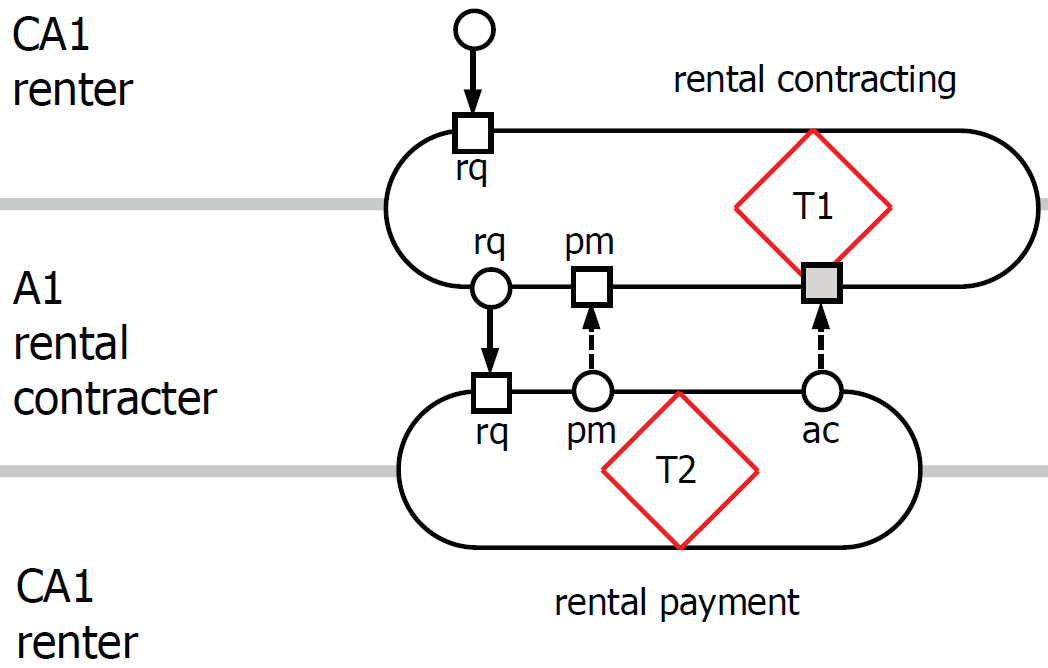
\includegraphics[width=6cm, keepaspectratio]{img/rac-psd-one} }}%
 \qquad
 \subfloat{{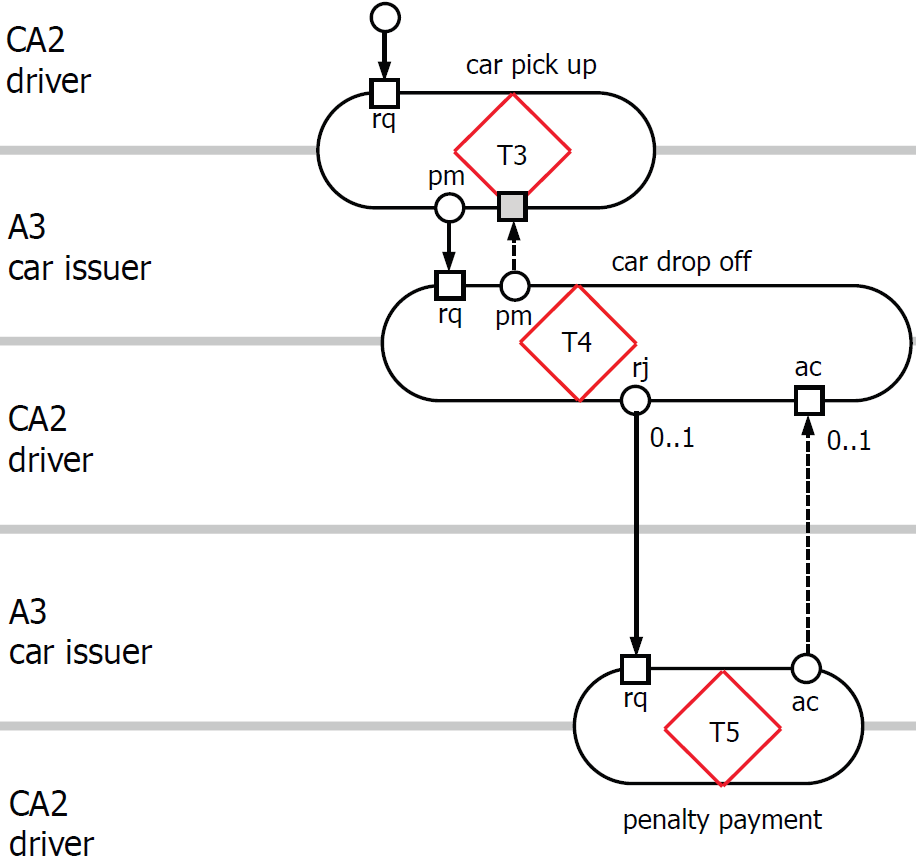
\includegraphics[width=6cm, keepaspectratio]{img/rac-psd-two} }}%
 \caption{RAC PSD}%
 \label{fig:rac-psd}%
\end{figure}
\newpage
% ----------------------------------------------------------------------------------------
\section{Data Labelling}
As has been said, every system within enterprise provides some collection of data. Problem is, if enterprise does note use centralized solution (a some form of \gls{bpms}), format of collected data can be very different. 
However collected data can be structured and then processed via procedure, named ``labelling''. Every system can provide collected data with some structured form. Then sooner defined \textit{Data Aggregation Service} must have mechanism how this structure map to defined \gls{demo} model. This mechanism will be for every enterprise and theirs systems unique, however fundamental idea and work-flow is the same.

Firstly used terms are defined:
\begin{description}
\item[log] -- The structured collected data from enterprise systems
\item[case id] -- The defined process.
\item[creation timestamp] -- Timestamp when created.
\item[end timestamp] -- Indicates end of given task.
\item[activity] -- An activity (task) within case.
\item[resource] -- An resource associated with activity. Typically an user.
\item[role] -- An user role which invoked an activity.
\end{description}

\Cref{tab:rac-log} is an shortened log from \textit{Rent-A-Car} company. The ``case id'' is equal to 1 (which is generally some internal identifier) and it is omitted from table. Also timestamps are omitted because they are not, for now, important.  

There are several activities, resources and roles. ``Labelling'' mechanism must distinguish each one of activities and assign appropriate \textit{Transaction} and \textit{Coordination-act} from \gls{demo} model. Also ``roles'' must be assigned to \textit{Actor roles} and ``resource'' is assigned as \textit{Actor}. An shortened example of ``labelling'' is shown at~\cref{tab:rac-log-labelling}. The ``role'' and \textit{Actor roles} are absolutely the same. 

\begin{table}[ht!]
\centering
\begin{tabular}{ | c | c | c | }
\hline
	\textbf{Activity} & \textbf{Resource} & \textbf{Role} \\ \hline
	Create Rental  Requisition & Peter Freeman & Renter \\ \hline
	Create Request for Payment & Alice Gree & Rental Contracter \\ \hline
	Payment Promise & Peter Freeman & Renter \\ \hline
	Analyse Rental Requisition & Alice Gree & Rental Contracter \\ \hline
	Make a Payment & Peter Freeman & Renter \\ \hline
	Accept Payment & Alice Gree & Rental Contracter \\ \hline
	Create a New Contract & Alice Gree & Rental Contracter \\ \hline
	Hand Over Contract to Customer & Alice Gree & Rental Contracter \\ \hline
	Customer Accepted Contract & Peter Freeman & Renter \\ \hline
	Create Car Pick Up  Requisition & Peter Freeman & Driver \\ \hline
    \multicolumn{3}{|c|}{\dots} \\ \hline
    
% 	Acquire Car Pick Up Request & Bob Hershel & Car Issuer \\ \hline
% 	Create Car Drop Off Requisition & Bob Hershel & Car Issuer \\ \hline
% 	Drop Off Requisition Agreement & Peter Freeman & Driver \\ \hline
% 	Car Preparation & Bob Hershel & Car Issuer \\ \hline
% 	Car Prepared for Pick Up & Bob Hershel & Car Issuer \\ \hline
% 	Driver Acquired the Car & Peter Freeman & Driver \\ \hline
% 	Customer Returning the Car & Peter Freeman & Driver \\ \hline
% 	Customer Returned the Car & Peter Freeman & Driver \\ \hline
% 	Car Returned & Bob Hershel & Car Issuer \\ \hline  
\end{tabular}
\caption{An example log of Rent-A-Car company}
\label{tab:rac-log}
  
\begin{tabular}{ | c | c | c | }
\hline
	\textbf{Activity} & \textbf{Transaction} & \textbf{State} \\ \hline
	Create Rental  Requisition & T1 & Request \\ \hline
	Create Request for Payment & T2 & Request \\ \hline
	Payment Promise & T2 & Promise \\ \hline
	Analyse Rental Requisition & T1 & Promise \\ \hline
	Make a Payment & T2 & State \\ \hline
	Accept Payment & T2 & Accept \\ \hline
	Create a New Contract & T1 & Execute \\ \hline
	Hand Over Contract to Customer & T1 & State \\ \hline
	Customer Accepted Contract & T1 & Accept \\ \hline
	Create Car Pick Up  Requisition & T3 & Request \\ \hline
    \multicolumn{3}{|c|}{\dots} \\ \hline
% 	Acquire Car Pick Up Request & T3 & Promise \\ \hline
% 	Create Car Drop Off Requisition & T4 & Request \\ \hline
% 	Drop Off Requisition Agreement & T4 & Promise \\ \hline
% 	Car Preparation & T3 & Execute \\ \hline
% 	Car Prepared for Pick Up & T3 & State \\ \hline
% 	Driver Acquired the Car & T4 & Accept \\ \hline
% 	Customer Returning the Car & T4 & Execute \\ \hline
% 	Customer Returned the Car & T4 & State \\ \hline
% 	Car Returned & T4 & Accept \\ \hline
\end{tabular}
\caption{Activities labelling from RAC log}
\label{tab:rac-log-labelling}
\end{table}
\clearpage
% -----------------------------------------------------------------------
\section{Process Instance Visualisation}
System must have ability to visualise running process instances in real-time. User can open running process and can be informed how it continues. 

The biggest challenge was how to propose a way to visualise models modelled with \gls{demo}. Moreover, the intent was mainly to provide visualisation on mobile devices (smart-phones, tablets).

There are four conditions how visualisation must be proposed:
\begin{enumerate}
	\item The proposed way must preserve the intention of modelled model through \gls{demo}.
    \item Visualisation must be consistent accordingly to defined \gls{demo} model.
    \item The proposed way must be easy to use and understand.  
    \item It must be adaptive to different sizes of mobile devices. 
\end{enumerate}

The first idea of visualisation was highly inspired from investigated existing solutions (\textit{Process Maker}, \textit{Bizagi Modeler}). Visualisation could be done with \gls{demo} \gls{ocd} model itself. With this approach user could have:
\begin{enumerate}
  \item The exactly same understanding of modelled enterprise.
  \item The straightforward visualisation of instances through defined models. If user understand \gls{demo} models, this approach of visualisation has the same meaning.
\end{enumerate}

With this approach first two conditions are accomplished:
\begin{enumerate}
\item Defined enterprise is directly exposed with \gls{ocd} model. However some information are hidden. As is known, the \gls{psd} brings more information how processes are defined and how they work. (i).
\item Consistency is tied with \gls{ocd} itself (ii).
\end{enumerate}

However the (iii) and (iv) are not so straightforward. The third condition (iii) is not accomplished because DEMO is used and it does not have to be easy to use and understand. In every enterprise there are specialists (business analysts) that have the responsibility to analyse given enterprise and specify models (for example within \gls{demo}). Other people do not need to have knowledge about this methodology, overall they do not need to have knowledge about some models either. Although \gls{ocd} itself is very concise, it is not so suitable to smaller screens of mobile devices. This implies, that also (iv) is violated.
% ----------------------------------------------------------------------------------------
\section{A Better Option}
Gantt chart is widely used in time-management projects and systems. It is well known, established and used. It was found, that Gantt chart offers the best approach, how tasks can be visualised. Chosen approach is highly inspired from it and visualisation is based on it. 

The visualisation is divided to two parts:
\begin{enumerate}
\item The ``Gantt-chart canvas'' where each transaction has own form of progress bars which displays transaction's current state.
\item Time-line which offers chronological overview which events occurred and when. 
\end{enumerate}
% ----------------------------------------------------------------------------------------
\subsection{Transaction Box Element}
Transaction box is associated rectangle with transaction which indicates current state of transaction. The state corresponds to actual C-Act within \textit{Transaction Pattern}. Current state also indicates progress value which is displayed as inner rectangle inside transaction box filled with colour. Progress value is computed as percentage value from current state. The C-Act \textit{Request} corresponds to 10 \%, \textit{Promise} to 25 \%, \textit{Execute} to 50 \%, \textit{State} to 75 \% and so on.  

The transaction box has four colour stages. \textbf{White} for not requested transaction yet (the box has also dashed border), a \textbf{green} which indicates ``happy path'' through \textit{Transaction Pattern}, a \textbf{yellow} if transaction is \textit{rejected} or \textit{declined} and \textbf{red} for transaction which is \textit{stopped} or \textit{quitted}. 

The transaction boxes are placed accordingly to \gls{ocd} model. That means:
\begin{itemize}
\item The transaction which ``starts'' whole process is placed as first. 
\item If transaction is dependent on another, it is placed ``under'' it and shifted to the right. Also that means, that ``parent'' transaction is wider than their descendants. 
\end{itemize}
% ----------------------------------------------------------------------------------------
\subsection{Transaction Link Element}
As has been said, \gls{psd} model defines associations between transactions. Each transaction can have many \textit{response} links and \textit{waiting} links. For better understanding, how process is defined, these links are within visualisation included. 

The links appearance is taken from \gls{psd} itself. 
\begin{itemize}
\item Response link is displayed as straight line with arrow at the end. On one side it has circle with \textit{source} C-Act, on the other side with arrow it has square with \textit{target} C-Act.
\item Waiting links is displayed as response link, but line between is dashed. 
\end{itemize}

Links are placed between appropriate transactions accordingly to \textit{source} and \textit{target} C-Acts, just like at \gls{psd}. However, if \textit{response} link has \textit{target} C-Act as ``Requested'', the abbreviation of \textit{target} is omitted and link itself is displayed as angled arrow which points to ``start'' of \textit{target} transaction. It is totally clear, that this type of response means exactly ``If given C-Act at  source transaction occurred then target transaction is also requested''.

Example shown at \cref{fig:box-state-state} means exactly: ``When transaction T1 is \textit{promised}, T2 is \textit{requested}. Then T1 can be \textit{stated} only if T2 was already \textit{promised}. Also T1 can be \textit{accepted} only if T2 was \textit{stated}.''

\begin{figure}[ht!]
\centering
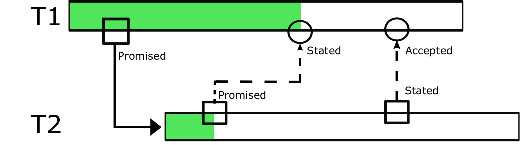
\includegraphics[width=9cm,keepaspectratio]{img/box-links-example}
\caption{The transaction links example}
\label{fig:box-state-state}
\end{figure}

On the canvas's left side are placed transaction labels. Label corresponds to transaction's name and identifier. The labels are structured to tree-form like in folder explorer. Each transaction box has same height position as corresponding label. 

With this approach, user has quick and easy way how can check state of concrete process. User can easily determine which transactions are not yet completed and how they are connected  together. 

However the time-based information still missing and that is the point, where time-line comes in.
% ----------------------------------------------------------------------------------------
\subsection{Time-line}
Main purpose of time-line is to provide chronological overview of incoming events. The time-line is scalable. This means, that user can zoom in or out to level of details. Typically more events can occur within one minute, so it is important to have ability to zoom to more detailed view. 

Each event is marked with timestamp (when event occurred) and what kind of event it is. If event is kind of ``C-Act occurred'', event has also information about associated transaction with C-Act's abbreviation. To help user more easily distinguish which transaction is associated with given event, each transaction has own colour, that is reflected to colour of text within time-line. 

Time-line is independently controllable and provide another point of view to the state of current running process. 

One note aside, the first idea was to provide connected associations between time-line and transaction boxes. The intent was to provide visuals (anchors) within transaction box that could indicate that ``at this point something happened''. If the user `click'' on this anchor then a visual connection between anchor and associated event within time-line appears. 

With this approach, the canvas must be capable of responding to time-line ``stretching'' -- transaction box must resize accordingly to positions of events within time-line. Although it makes perfectly sense from user ``point-of-view'', the usability within mobile-devices is reduced. Each event within time-line must be readable and with adding of events, width of transaction box grows. Result is, that each transaction box is really wide and it becomes very unclear and nearly unusable.

Resulting approach can be summarized as follows:
\begin{itemize}
\item The visualisation is divided to two views.
\item First one, the time-line offer chronological overviews of occurred events associated with transactions.
\item The second one offers the overview current transactions states and the associated links between them. 
\end{itemize}
% ----------------------------------------------------------------------------------------
\section{The Dashboard}
Although the ``process visualisation'' brings usable kinds of overviews, there are many types of overviews which can't be done through this. As has been said in \cref{ch:bpms}, typical \gls{bpm} solutions offers some kind of ``dashboard'' where these various types of overviews are placed together. 

The dashboard's main goal is to provide:
\begin{enumerate}
\item The comprehensive and effective way how to get precious information over collected data.
\item Ability to provide highly customized and individual types of overviews. A company will want to propose a different overviews for sales manager than for accountant and so on. 
\item The overviews must be easy to understand and must be very clear, what they display.
\end{enumerate}

\subsection{Data Query}
To provide a specific view over collected data, it is required to collected data be specifically aggregated according to defined overviews. For this purpose, the \textit{data query} is defined.

\textit{Data Query} is basically named query over collected data. This also can be also compared as ``stored-procedure'' within DBMS (Database Management System). From end-user point of view, user only select defined query and data are returned. Within \textit{Data Aggregation Service} query is defined and transformed to ``real'' query over collected data. In most of cases, it will be transformed to SQL-like query. 

Within \gls{bpm} solution (based on \gls{demo}) is defined \textit{query editor}. It is simple, form-based editor, where employees within an enterprise can define \textit{data queries}. User defines \textit{name} of query and builds the query with interactive guide. For simplicity, the guide can be imagined as interactive way how to build a SQL query with clauses as ``join, where, group by, order by, etc.''. Result is, that editor allows to non-technical users still define basic queries over collected data without requirement to have knowledge, how concretely ``grab'' the data in technical way. 

Each overview within dashboard is called \textit{widget}. Widgets provide one concrete type of view. Widgets has defined \textit{name} and associated \textit{data query}. Each widget is highly customisable, but they are sorted to a several base types.

\subsection{Summary Widget}
The summary widget provides, by its name, summarization about collected data. It is commonly displayed as ``Pie chart''. The typical usage for example can be: ``Summary of ratio between Accepted and Declined contracts'' or ``Actual state of all contracts, number of requested, stated, declined, accepted and so on'',~\dots

\subsection{Time Based Widget}
This widget displays data between defined time period. It uses ``Column chart''  (each \textit{time x-value} is displayed as column with height of \textit{y-value}) or ``Line series chart''. An example of typical usage can be: ``Monthly income-expense'', ``Daily number of new contracts'',~\dots

\subsection{Single Value Widget}
An single value computed from collected data. This can be for example ``Actual number of unresolved contracts'', ``Actual financial balance'',~\dots 

\subsection{Widgets As Placeable Elements}
Dashboard can be divided to ``grid layout'' -- a unspecified number of rows and from one up to three columns. Each widget has defined the \textit{width} and the \textit{height} -- how many columns and rows it will take. The the user can simply arranges widgets exactly how he wants.


\section{\todo{Graphs as Widgets, Dashboard}}
\section{\todo{Queries and editor}}
\section{\todo{A Few More Ideas of Visualisation}}
%     \section{Overviews}
    
%     \section{Process visualization}
    
%     \section{Mobile application concept}
	
% 	\todo{Domain model of collected data. Proposed way of real time visualization. Type of charts. Dashboard. Whole concept of application, e.g dashboard, editor. Functional specification, a.k.a example use cases?? Domain model of collected data.}
    
%     \section{Analysis}    

   

% 	\section{The dashboard}
%     Purpose of dashboard is provide centralized overview of processes such as average waiting time before process is completed or total amount of requests per day. The appearance of dashboard depends on user. \gls{dwma} provides customizable elements called widgets to achieve desired look for every user individually.

%     \subsection{Widgets}  
%      Widgets are small independent configurable components for displaying collected data from business processes. Each one has purpose. Notice that widgets are only user-friendly view of query above collected data. For editing widgets there is widget editor. User can simply edit properties of widget such as name, category, tags and of course source of data - the query and second important property is the type of widget. There are following types of widgets:
     
%      \textbf{The summary widget} (\cref{fig:widget-summary}) provides, by it's name, chart with summarization of collected data. Concrete type of the chart depends on the user and on the data. Summary widget provides several types of charts:
     
%      \begin{enumerate}
%     	\item \textit{Pie} chart is used to illustrate numerical proportion.         
%         \item  \textit{Bar} chart displays categorical data with numerical value.
%         %\item \textit{Line}
%     \end{enumerate}
      
%       \begin{figure}[ht!]
%           \centering
%           
\includegraphics[width=6cm,keepaspectratio]{img/TODO-image}
%           \caption{Summary widget example}
%           \label{fig:widget-summary}
%       \end{figure}   
    
%    	Second type is \textbf{Time period} (\cref{fig:widget-time-period}). Time period displays data in some interval. Typically it can serve as overview \textit{``Number of requests for Rental payment per day"}.        
      
%       \begin{figure}[ht!]
%           \centering
%           
\includegraphics[width=6cm,keepaspectratio]{img/TODO-image}
%           \caption{Time period widget example}
%           \label{fig:widget-time-period}
%       \end{figure}
    
%     Last type is \textbf{Single query} (\cref{fig:widget-single-query}) which allows display simple result from query. Prerequisite for query is that query returns one single record. 
      
%       \begin{figure}[ht!]
%           \centering
%           
\includegraphics[width=6cm,keepaspectratio]{img/TODO-image}
%           \caption{Single query example}
%            \label{fig:widget-single-query}
%       \end{figure}       
    
%     \subsection{Query editor}
    
%     \todo{Information about query editor}
    
%     \begin{figure}[ht!]
%           \centering
%           
\includegraphics[width=6cm,keepaspectratio]{img/TODO-image}
%           \caption{\todo{Query editor}}
%       \end{figure}   
    
%     \section{The real-time overview of process instance}
%     \todo{Introduction about gantt chart. Make conversation about classic OCD / PSD diagrams and their pros and cons for visualizations}
%     Provides the real-time overview of one concrete process instance.
% On the left side is tree-view (like in folder explorer) of transactions. Each transaction has identifier and name.
% On the top is the timeline which displays important events from the process. Above timeline is visualization itself. Each transaction is displayed as progress bar with some visual tweak, which will be discussed later.

% 	Each transaction can be at one of the following state, which has different visual: 
% 	\todo{Categories}
    
%     \begin{description}
%     	\item[Not active transaction] Is displayed as greyed out progress bar. It means that this instance of transaction will be probably started at some future time.

%         \item[Active transaction] Progress bar is displayed with green colour to show current progress of instance transaction. 
        
%         \item[Completed transaction] Progress bar is fulfilled with green colour. It means that given transaction successfully ended (was accepted).
        
%         \item[Stopped transaction] Progress bar changed colour to red which indicates that transaction failed to complete due to fact that it was quitted or stopped. 
%     \end{description}
    
%  \subsection{Response and waiting links}
%     \todo{Change this}
%    Each transaction can have several child-transactions and also many conditional links. These conditions are displayed with arrows pointed to another transaction with the condition.
% Conditions are divided into two categories.

% If the condition is ``Some state of transaction A has to be done before transaction B can start (be requested)", e.g. transaction A must be stated before transaction B can be requested (\cref{fig:request-start-condition}).

% \begin{figure}
%   \centering
%   
\includegraphics[width=6cm,keepaspectratio]{img/TODO-image}
%   \caption{\todo{Request-start condition}}
%   \label{fig:request-start-condition}
% \end{figure}  

% If condition is ``Some state of transaction A has to be done before transaction B can be at another state", e.g transaction A must be at least stated before transaction B can be promised (\cref{fig:state-state-condition}).

% \begin{figure}
%   \centering
%   
\includegraphics[width=6cm,keepaspectratio]{img/TODO-image}
%   \caption{\todo{State-state condition}}
%   \label{fig:state-state-condition}
% \end{figure}  



\chapter{Proof of Concept}
\label{ch:proof-of-concept}
\todo{Used technologies. Brief description of Xamarin, Signal R, .NET standard / .NET Core, XAML, ASP .NET Core.Screens, screens :)Good explanation how state of implementation is so "bad". Problems with Xamarin, SIgnalR, incompatibility. And heck, the whole implementation of Gantt chart...}

To verify proposed approaches, the simple mobile application as proof-of-concept was implemented. To verification was chosen especially process instance visualisation.

The given application offers:
\begin{enumerate}
\item Process instance visualisation with simulated data
\item Concept of dashboard
\end{enumerate}

In this chapter, firstly the used technologies are introduced. Then the brief architecture of mobile application and implementation itself are explained. In the end, the
% ---------------------------------------------------------------------------------
\section{.NET Platform}

For implementation is used .NET platform and programming language C\#. The .NET is free, open-source and cross-platform framework for building many different types of applications \todo{cite}. There is a lot of frameworks within platform, such as WPF for building native desktop applications for Windows or ASP .NET framework for building websites and server-side applications. Also there is cross-platform Xamarin framework for building mobile applications. These all frameworks were used to implement proof-of-concept. 
% ---------------------------------------------------------------------------------
\subsection{.NET Standard}
\begin{figure}[ht!]
\centering
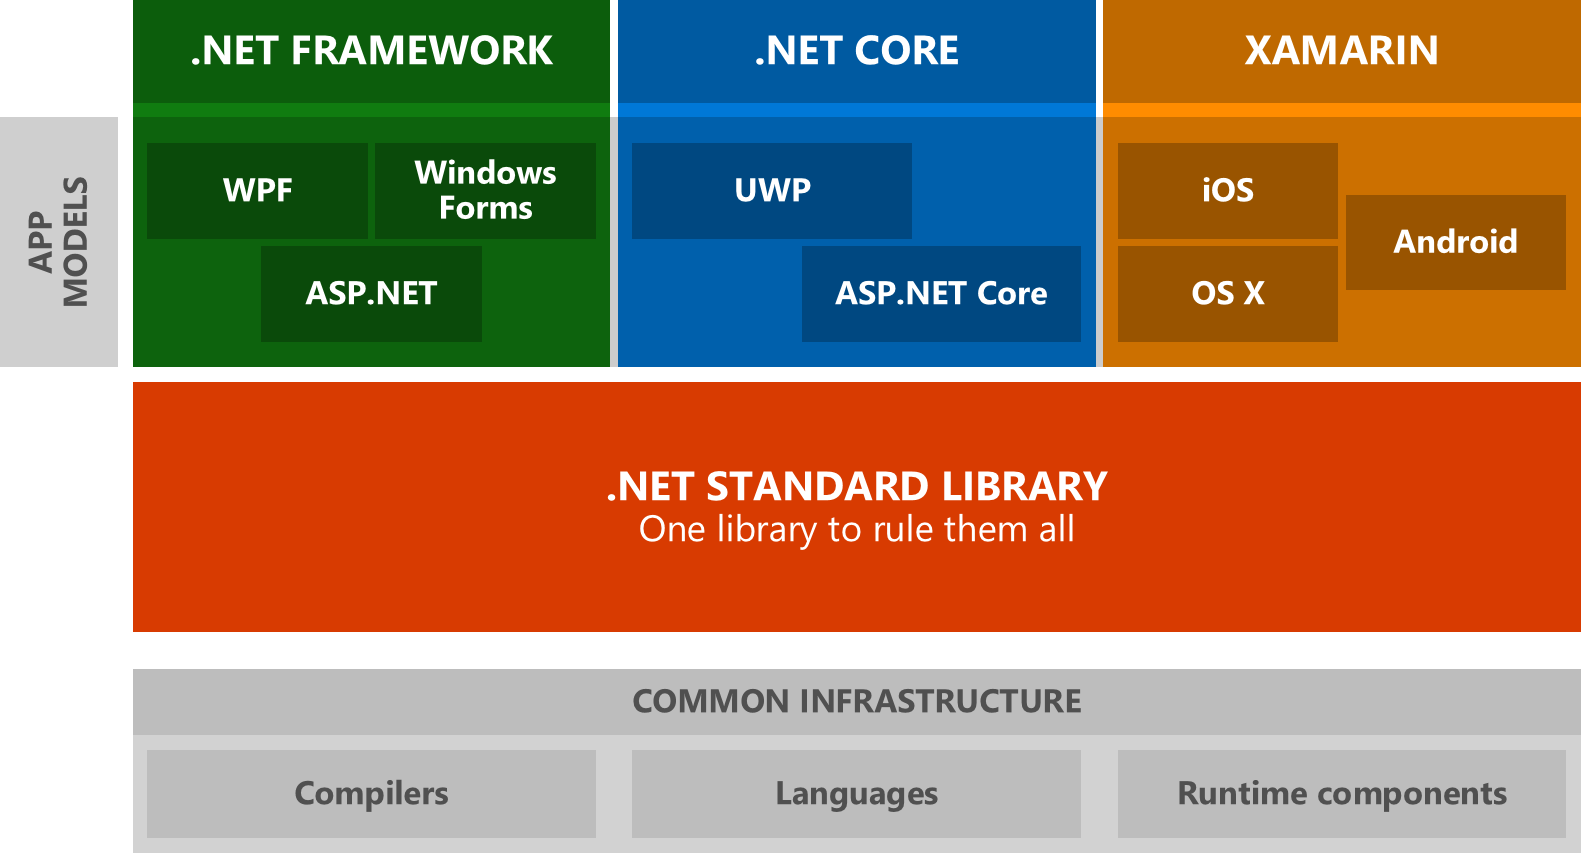
\includegraphics[width=12cm,keepaspectratio]{img/dotnet-overview}
\caption{The .NET platform overview \cite{introducing-dotnet-standard}}
\label{fig:dotnet-overview}
\end{figure}

Earlier years within .NET platform was problem with many different implementations of .NET itself. There was the ``original'' (full) .NET. Then a newer, open-source and cross-platform version .NET Core and third was Xamarin. Each platform have different base libraries and if developers wanted to share code between these platforms, there was a lot of work to do. 

The new approach was introduced \cite{introducing-dotnet-standard}, the .NET Standard -- the unified platform which defines set of APIs that each .NET subset platform must implement. This allows to developers easily share code and write libraries that can be used anywhere. The great graphical summarization is shown at \cref{fig:dotnet-overview}. Actual version is .NET Standard 2.0. The newer version 2.1 will be introduced within Q2 2018. 
% ---------------------------------------------------------------------------------
\subsection{.NET Core}
The .NET Core is open-source, cross-platform version of .NET Framework. It is new and highly frequently updated framework which becomes very popular. It has many ``ports'' of frameworks from full .NET such as ASP .NET or Entity Framework -- an Object-Relationship-Mapping tool for databases. 
% ---------------------------------------------------------------------------------
\section{Xamarin}
Xamarin is platform for developing native mobile applications in cross-platform way. Developers use C\# language and .NET Standard to implement mobile application. When the application is being build, the code is compiled to native platform code. 

Following summarization is taken from \cite{xamarin-understand-platform}:
\begin{itemize}
\item On iOS, C\# is ahead-of-time (AOT) compiled to ARM assembly language. The .NET framework is included, with unused classes being stripped out during linking to reduce the application size. Apple does not allow runtime code generation on iOS, so some language features are not available.
\item On Android, C\# is compiled to IL and packaged with MonoVM. Unused classes in the framework are stripped out during linking. The application runs side-by-side with Android runtime.
\item Windows and UWP use directly C\# and included .NET. 
\end{itemize}

Within Xamarin there are two main approaches how to build applications (see \cref{fig:xamarin-native-vs-forms}). First one is commonly called ``Xamarin Native'' or ``Xamarin.*'' where * is targeted platform. With this approach, the code for business logic is written independently from target platform, but user interface for each platform is implemented separately with native approaches (e.g. for Android developer uses XML based declarations).

\begin{figure}[ht!]
\centering
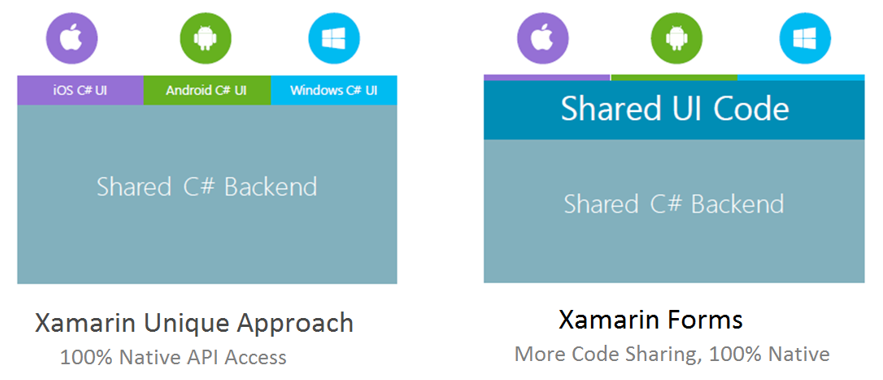
\includegraphics[width=12cm,keepaspectratio]{img/xamarin-vs-xamarin-forms}
\caption{The Xamarin.* vs Xamarin.Forms \cite{xamarin-native-forms}}
\label{fig:xamarin-native-vs-forms}
\end{figure}

\begin{figure}[ht!]
\centering
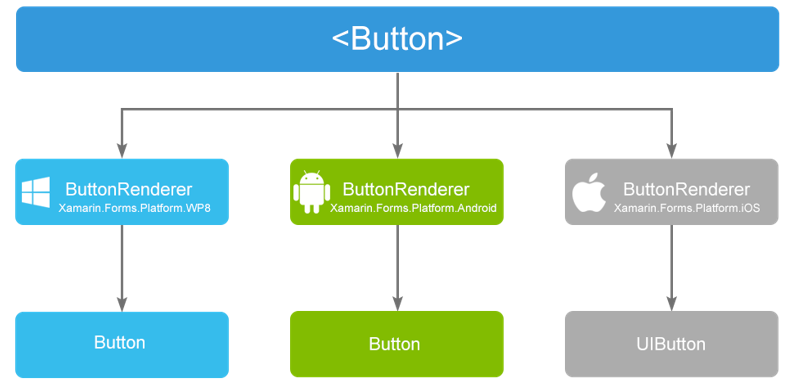
\includegraphics[width=10cm,keepaspectratio]{img/xamarin-forms-ui-render}
\caption{The Xamarin.Forms control renderer \cite{xamarin-native-forms}}
\label{fig:xamarin-ui-renderer}
\end{figure}

Second one is called Xamarin.Forms, which is build on top of first one and allows to define user interfaces in cross-platform way. Developers use XAML, the declaration language similar to XML to define user interface. When application is being build, defined controls are transformed to native controls. This transformation is done through concept called ``Control renderer''. Within shared library, an interface for control is defined. On each platform is implemented render which transforms given control to native one. An example is shown at \cref{fig:xamarin-ui-renderer}.
% ---------------------------------------------------------------------------------
\section{Another Used Technologies}
The implementation is divided to two parts. First one is mobile application and second one is server-side, the concept of \textit{Data Aggregation Service}. 

For server-side implementation was chosen ASP .NET Core -- a newer version of ASP .NET, framework for creating server applications  (services, REST API, \dots) and websites.

Within ASP .NET Core a web application was created and library SignalR was chosen.
% ---------------------------------------------------------------------------------
\subsection{SignalR}
\begin{figure}[ht!]
\centering
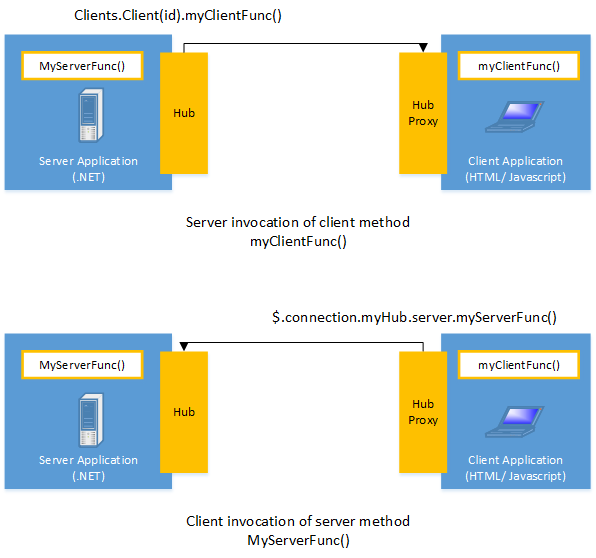
\includegraphics[width=8cm,keepaspectratio]{img/signal-r-overview}
\caption{How SignalR works \cite{signal-r-overview}}
\label{fig:signal-r-overview}
\end{figure}
According to \cite{signal-r-overview} SignalR is: ``a library for ASP .NET which offers adding real-time web functionality to applications. Real-time web functionality is the ability to have server code push content to connected clients instantly as it becomes available, rather than having the server wait for a client to request new data''. SignalR handles ``many things'' for developers automatically, such as connection management or choosing transporting types. SignalR firstly try to use WebSocket and if it fails, automatically fall back to older transports.

On the server, developer defines a \textit{Hub}. Hub defines contract which clients will use and communicate through. On the client-side, developers creates \textit{Hub Proxy} -- connection to specific \textit{Hub}. An example how it works is shown at \cref{fig:signal-r-overview}.
% ---------------------------------------------------------------------------------
\section{Implementation Choices}
For implementation were chosen a quite new and interesting technologies and combinations of them.
The .NET Standard is for now the only one right way how to create shared C\# back-end. Older approaches with Portable Class Libraries (PCL) are deprecated and Xamarin recommends to use .NET Standard. Although it is recommended and PCL are deprecated, many problems occurred. More discussion about problems with implementation is in the end of this chapter.

For mobile-application was chosen Xamarin.Forms for this reasons:
\begin{itemize}
\item Author has many experiences with XAML from similar frameworks such as WPF or Universal Windows Platform.
\item Xamarin.Forms are more faster for developing with cross-platform way -- the user interface is written once.
\end{itemize}

Xamarin.Forms offers many prepared controls for use, but for creation of process instance visualisation a custom control were created.  

A many different approaches were tried. First one was to edit already exists controls, but it comes, that it is not suitable. Another approach was to find existing controls, which resulted to, that the requirements are too specific. Third option was to use some basic 2D engine for custom drawing and rendering. The third option seemed as best option to do, so it was chosen. 

\subsection{SkiaSharp}
SkiaSharp library \cite{skiasharp} provides a way how to quickly and easily do custom 2D drawing. It is used for process visualisation. Each \textit{transaction box} is custom control created with SkiaSharp's canvas -- a place-holder for custom drawings. Each \textit{transaction link} and events on timeline are also custom controls made with this library. 

\subsection{SyncFusion Controls Library}
SyncFusion Controls Library \todo{cite} adds many new controls to Xamarin.Forms. The Dashboard uses this library for its various types of charts. 

\subsection{Simulation Cases}
Main goal of proof-of-concept is to verify that proposed visualisation approach is usable. In real-world usage, many other systems and services must be developed. Also, there is not any ``real-world'' data source. So, the simulation approach was chosen. As base model was chosen Rent-A-Car company. Above that, a several simulation cases are prepared. 

\section{Implementation Details}
Only fundamental implementation decisions and circumstances are described. At the \cref{fig:impl-dependecies-graph} is shown ``high-level'' architecture of application. 

\begin{figure}[ht!]
\centering
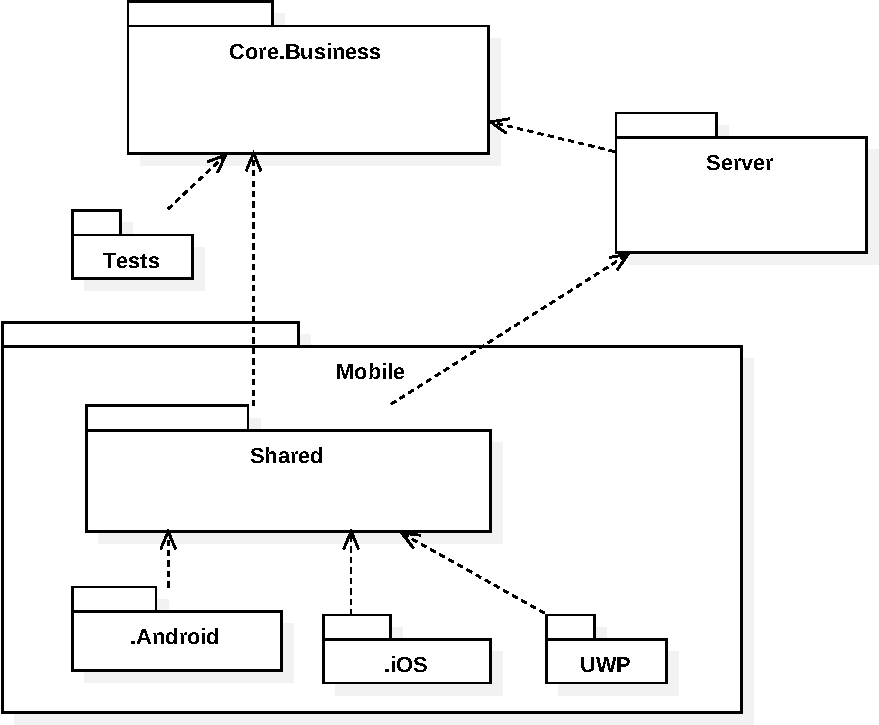
\includegraphics[width=10cm,keepaspectratio]{img/dependecies-graph}
\caption{The implementation packages}
\label{fig:impl-dependecies-graph}
\end{figure}

\begin{description}
\item[Core.Business] -- The \textit{Data Domain Model} is placed here, because mobile and server applications use it. Also classes for simulations and XML parsers are there.
\item[Server] -- The simple ASP .NET Core with SignalR application for serving a simulation data.
\item[Mobile.Shared] -- A shared part of Xamarin application. All business logic and user interface are implemented here.
\item[Mobile.Shared.Android] -- A Xamarin.Android project. There are Android specific implementations and boot-strapper for Xamarin.Forms on Android. Also all the graphic assets (logo, icons, \dots) are placed within this project.
\item[Mobile.Shared.iOS] -- A Xamarin.iOS project. Same purpose as Mobile.Shared.Android.
\item{Mobile.Shared.UWP} -- A Xamarin.UWP (Universal Windows Platform) project. Same purpose as Mobile.Shared.Android.
\item[Tests] -- Package contains several unit tests for Core.Business. 
\end{description}





\begin{conclusion}
	In the introduction and first two chapter were introduced theoretical foundations and showed existing BPM solutions which are commercially used. The goal of thesis was mainly propose a way how visualisation of processes defined within DEMO can be done. A few approaches were inntroduced. Than followed explanation why chosen approach is the best for the visualisation. 

The possibility of real usage was proofed through mobile application. The goal was to provide a simple to use and to understand approach, which seems to be accomplished. The visualisation is highly inspired from widely used Gantt charts, which are popular mainly in task-management. Also the concept of widgets within dashboard was described. These widgets provides user high valuable overview of collected data which can really help to improve their business. 

\subsection{Future steps}
A visualisation itself could be defined more universally and could provide a detailed approach how any enterprise system can be mapped to defined DEMO models. As has been noted, a few existing solution based on DEMO exists. The really next step could be to include this visualisation  approach into existing BPM solutions based on DEMO. Thanks to this step a complete BPM solution could exists.
\end{conclusion}

\bibliographystyle{iso690}
\bibliography{myref.bib}

\appendix

\printglossaries

\chapter{Content of Enclosed CD}

%upravte podle skutecnosti

\begin{figure}
	\dirtree{%
		.1 readme.txt\DTcomment{Brief description of  CD content}.	
		.1 src.
		.2 impl\DTcomment{implementation source code}.
		.2 thesis\DTcomment{\LaTeX{} source code of text}.
		.1 text.
		.2 thesis.pdf\DTcomment{Thesis text in PDF form}.
	}
\end{figure}

\end{document}
